\documentclass[a4paper,11pt]{article}


\usepackage{minted}
\usepackage{amsmath}
\usepackage{amssymb}
\usepackage{amsthm}
\usepackage{graphicx}
\usepackage{enumerate}
\usepackage{xcolor}
\usepackage{biblatex}
\usepackage{rotating}
\usepackage{algorithm}
\usepackage{algpseudocode}
\usepackage{pdflscape}

\usepackage[UKenglish]{babel}
\usepackage{csquotes}

\usepackage[hidelinks]{hyperref}
\hypersetup{
    colorlinks=false, %set true if you want colored links
    linktoc=all,     %set to all if you want both sections and subsections linked
    linkcolor=black,  %choose some color if you want links to stand out
}


\addbibresource{percolation.bib}

%------------------

%\setlength{\topmargin}{0.0in}
%\setlength{\textheight}{10in}
%\setlength{\oddsidemargin}{0.0in}
%\setlength{\evensidemargin}{0.0in}
%\setlength{\textwidth}{6.5in}

%-------------------
\newtheorem{theorem}{Theorem}[section]
\newtheorem{proposition}[theorem]{Proposition}
\newtheorem{lemma}[theorem]{Lemma}
\newtheorem{corollary}[theorem]{Corollary}
\newtheorem{conjecture}[theorem]{Conjecture}


\theoremstyle{definition}
\newtheorem{definition}[theorem]{Definition}
\newtheorem*{example}{Example}
\newcommand{\ints}{\mathbb{Z}}
\newcommand{\sigalg}{$\sigma$-algebra }
\newcommand{\ztwodual}{(\ints^2)^*}
\newcommand{\prob}{\mathbb{P}_p}
\newcommand{\expp}{\mathbb{E}_p}
\newcommand{\prbhlf}{\mathbb{P}_{1/2}}
\newcommand{\probtorus}{\mathbb{P}^{\mathbb{T}}_{p}}
\newcommand{\probtorush}{\mathbb{P}^{\mathbb{T}}_{1/2}}
%------------------

%Everything before begin document is called the pre-amble and sets out how the document will look
%It is recommended you don't touch the pre-amble until you are familiar with LaTeX

\begin{document}
\thispagestyle{empty}

\begin{figure}[h]
\begin{center}

\includegraphics[scale=0.5]{uob.pdf} %make sure the pdf file named 'uob' is saved in the same folder as this file
\end{center}
\end{figure}

\begin{center}
{\Large Percolation\\ \vspace{1cm}Jonathan Marriott}
\end{center}

\vspace{3cm}
\hrule
\begin{center}
Supervised by Dr Edward Crane\\
Level 6\\
20 Credit Points
\end{center}
\hrule

\vspace{3cm}
\begin{center}
\today
\end{center}
	
\title{Percolation}
\author{Jonathan Marriott}
\date{}
\maketitle

% \begin{abstract}
% Some sorts of documents need abstracts. Others do not.
% \end{abstract}

%The following code is not run because of the percentage sign, but you might find it useful for future work
\tableofcontents{}



\section{Introduction}
Originally the percolation model was devised to capture the physical properties of liquids flowing through porous mediums. The model introduced in 1957 by Broadbent and Hammersley \cite{broadbent_hammersley_1957} has produced a rich mathematical theory with wide-ranging applications in areas including disease spread \cite{meyers2007contact}, network robustness \cite{callaway2000network}, ferromagnetism \cite{aizenman1991strict} and forest fire spread \cite{stauffer2018introduction}.
In this report we first introduce the percolation model, with no expectation on the reader to have a strong understanding of measure theory nor probability theory as the necessary definitions are included here. Subsequently, our main aim is to prove a key result in percolation theory - the Harris-Kesten Theorem. This theorem tells us the point at which percolation on the square lattice undergoes its phase transition, notably percolation is  one of the simplest mathematical models to exhibit such behaviour. Finally, we look at percolation through the lens of computer simulations, to see how one might investigate the critical behaviour in unknown graph structures.


%Using the percentage symbol, you can include comments in your code that do not appear in the output.


% \section{Formatting}

% We can \emph{emphasis} some words, i.e., make them \emph{italic}, and we can make some words \textbf{bold}.
% Note how using a new line in the code does not correspond to a new line in the output file.
% Same if we have        a           large                white                   space.

% Instead, if we want a new line/new paragraph, you need to press enter twice, or use \\
% which starts a new line but not a new paragraph.

% \subsection{lists}

% Lists can be numbered or unnumbered, and you can have sub-list inside a list.

% \begin{enumerate}
% 	\item This is the first item in a numbered list.

% 	\item And the second
	
% 	\item 
% 	\begin{enumerate}
% 		\item Here the third item is in fact a numbered sub-list.
% 		\item item 2 of the numbered sub-list
% 	\end{enumerate}

% 	\item 
% 	\begin{itemize}
% 		\item Here the fourth item is an unnumbered sub-list.
% 		\item item 2 of the unnumbered sub-list
% 	\end{itemize}
% \end{enumerate}
\section{Introducing the Percolation Model}
Broadly percolation theory can be split into 2 main categories: bond percolation and site percolation. Given some initial graph, in site percolation instead we assign the vertices of the graph to be open or closed. Whereas in bond percolation we assign edges to be open or closed, see Figure~\ref{fig:simBox}. Due to historic reasons the terminology used in percolation theory differs from that used in modern graph theory. Where graph edges and vertices are often referred to as bonds and sites respectively. Throughout this report we will be largely focusing on bond percolation, although it is interesting to note that all bond percolation problems can be reformulated as site percolation problem but not always the other way around \cite{grimmett1999percolation}.

\begin{figure}
	\centering
	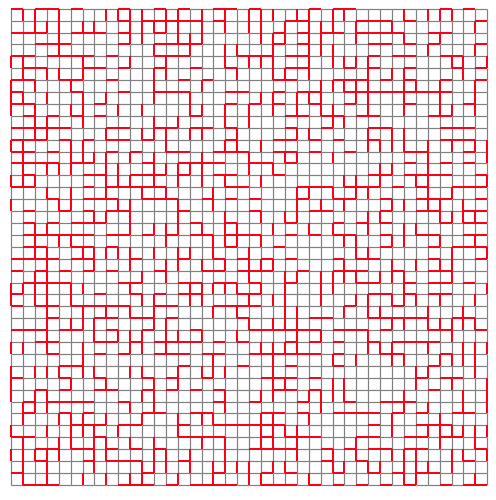
\includegraphics[scale=0.7]{drawings/simulationConfig.png}
	\caption{An example bond percolation configuration on a 40 by 40 box of the square lattice when $p=0.4$. Where red edges are open and grey edges are closed.}
	\label{fig:simBox}
\end{figure}
\subsection{Cubic Lattices}

We start by introducing some basic notation and definitions for cubic lattices. In general, we match the notation and definitions given in \cite{steif2011mini}. The measure and probability theory definitions given largely follow \cite{ash2000probability}, but we also use \cite{bollo2006} for percolation specific details.

\begin{definition}[Integers]\label{ints} 
	$\mathbb{Z} = \{...,-2,-1,0,1,2,...\}$ and $\mathbb{Z}^d = \{(x_1,x_2,...,x_d) : x_i \in \mathbb{Z} \}$
\end{definition}

\begin{definition}[1-norm distance]\label{dist}
	For $x,y\in \mathbb{Z}^d$, define the distance from x to y, denoted $\delta(x,y)$, by
	$$\delta(x,y) := \sum_{i=1}^{d}|x-y|$$
\end{definition}\label{lattice} 

\begin{definition}[d-dimensional cubic lattice]{
	We construct the d-dimensional cubic lattice with vertex set $\ints^d$ and edges between vertices at distance one.
	$$E(\ints^d) = \{\{u,v\}:u,v \in V(\ints^d),\: \delta(u,v) = 1\}$$
	We will often abuse notation and refer to d-dimensional cubic lattice by the vertex set $\ints^d$ without specifying the edge set.
	We will also denote the origin by $0$.
}
\end{definition}


\subsection{Probability Space}

We now introduce the measure theory basics required to define the probability measure and subsequently the probability space for our percolation model.

\begin{definition}[$\sigma$-algebra]
	For some set $X$, we call $\mathcal{A} \subseteq \mathcal{P}(X)$, a subset of the power set of X, a  $\sigma$-algebra of $X$ if:
	\begin{enumerate}
		\item $\emptyset,X \in \mathcal{A}$
		\item $A \in \mathcal{A} \implies A^c := X \setminus A \in \mathcal{A}$ (Closed under complement)
		\item For $A_i \in \mathcal{A}, i \in \mathbb{N}$ we have that $\bigcup^\infty_{i=1} A_i \in \mathcal{A}$ (Closed under countable unions)
	\end{enumerate}
	We call the pair $(X,\mathcal{A})$ a measurable space, and elements of $\mathcal{A}$ measurable sets.
\end{definition}

We note by De Morgan's Laws that a $\sigma$-algebra is also closed under countable intersections.

\begin{definition}[Measure]
	A measure $\mu$ on a measurable space $(X,\mathcal{A})$ is a function $\mu: \mathcal{A} \rightarrow [0,\infty]$ where 
	$\mu(\emptyset) = 0 $ and for disjoint $A_i \in \mathcal{A}$, $i \in \mathbb{N}$ we have that
	$$ \mu\left(\bigcup^\infty_{i=1} A_i\right) = \sum_{i = 1}^{\infty} \mu(A_i)  $$
	Then we call the triple $(X,\mathcal{A},\mu)$ a measure space.
\end{definition}

In the context above if we think about X being our set of outcomes, and the sigma algebra of X representing the set of events we wish to assign a probability to, it seems sensible to give these events a probability via measure. 
However, we clearly need to restrict our measure which assigns these probabilities such that its domain is the interval $[0,1]$ 

\begin{definition}[Probability Measure]
	Let $\Omega$ be the set of all outcomes (the sample space) and $\mathcal{F}$ be a \sigalg of $\Omega$ where the elements are events we wish to consider (the event space). Then a measure $\mathbb{P}$ on $(\Omega,\mathcal{F})$ is a probability measure if:
	\begin{enumerate}
		\item $\mathbb{P}: \mathcal{F} \rightarrow [0,1]$
		\item $\mathbb{P}(\Omega) = 1$
	\end{enumerate}
	Then we call the triple $(\Omega,\mathcal{F},\mathbb{P})$ a probability space.
	
\end{definition}

\subsection{The Percolation Model}

We now take some parameter $p \in [0,1]$, this will specify the probability any given edge is open. 
Setting $q = 1-p$ we say each edge is independently open with probability p and closed with probability q.
We can think of the open and closed edges defining a random subgraph of $\ints^d$ where only edges set to open are retained.

Now we define our sample space $$\Omega = \prod_{e \in E(\ints^d)} \{0,1\}$$ where an edge in state 1 represents it is open, and 0 that it is closed.\\
We may refer to $\Omega$ as the set of configurations, where a configuration $\omega \in \Omega$ is a function assigning edges to be open or closed, meaning 
\begin{align*}
	\omega:&E \to \{0,1\}\\
	&e \mapsto \omega_e
\end{align*}
Then we must define $\mathcal{F}$, some \sigalg of $\Omega$, the set events we wish to assign a probability to. 
Clearly we cannot just take $\mathcal{F} = \mathcal{P}(\Omega)$, since we have uncountably many configurations in $\Omega$. 
This can be easily seen via a diagonalization argument. 
It turns out we can generate the \sigalg we want by the cylinder sets of $\Omega$. We base our definition on the one given by \cite{bollo2006}.

\begin{definition}[Cylinder Set]
	We say a subset $S \subseteq \Omega$ is a cylinder set if and only if there exists a finite subset $F \subseteq E$ and $\sigma \in \{0,1\}^F$ such that 
	$$S(F,\sigma) = \{\omega \in \Omega: \omega_f = \sigma_f \text{ for }f \in F\}$$
	In essence the cylinder set is the set of configurations $\omega$ which map all the edges in F to the same state that $\sigma$ does.
\end{definition}

Then we define $\mathcal{F}$ to be the set of all unions of cylinder sets of $\Omega$, then $\mathcal{F}$ is said to be generated by the cylinder sets of $\Omega$.
In this case $\mathcal{F}$ is a \sigalg of $\Omega$. Intuitively $\mathcal{F}$ is the set of events which only depend on a finite number of edges.\\
Next we define our probability measure on $(\Omega, \mathcal{F})$ by 
$$\prob(S(F,\sigma)) = \prod_{f \in F} (p(\sigma_f) + q(1-\sigma_f)) $$
Where again $q = 1-p$, and we use the subscript $p$ in $\prob$ to emphasize that $p$ is the parameter in our model, such that later if we fix $p$ to a specific value it will be clear.
Notice that we have defined $\prob$ for cylinder sets rather than elements of the $\sigma$-algebra, however it turns out by
Carathéodory's extension theorem the probability measure above has a unique extension to the whole $\sigma$-algebra.
For the details of this theorem see Theorem~1.3.10 in \cite{ash2000probability}.
Then $(\Omega, \mathcal{F}, \prob)$ is our probability space in which we examine the percolation model.


We now lay out some definitions specific for percolation.
\begin{definition}
	Let $C(x)$ denote the open cluster (component) containing $x$, which is the set of vertices in $\ints^d$ which are connected to $x$ by a path of open edges.
	We abbreviate the open cluster containing the origin $C(0)$ by $C$
\end{definition}

\begin{definition}[Increasing Event]
	An event $ A \subseteq \Omega$ is increasing if when $\omega \in A$ and
	$$\forall e \in E(\ints^d) \text{, } \omega_e = 1 \implies \omega'_e = 1$$
	Then $\omega' \in A$. 
	\end{definition} 

	We notice that the event $\{|C| = \infty\}$ is clearly an increasing event, since adding open edges to a configuration with an infinite connected cluster containing the origin will not remove the infinite cluster.

\begin{definition}[Percolation function]
	We define the percolation function $\theta(p)$ as follows
	$$\theta(p) = \prob(|C| = \infty)$$
	In words the percolation function is simply the probability that we can reach an infinite number of vertices from the origin by open edges. 
	Furthermore, we also note that this is the same as asking what is the probability of having an infinite length self-avoiding path of open edges starting at the origin.
\end{definition}

We intend to show that this percolation function is non-decreasing, but first we show a more general result for increasing events.

\begin{lemma} \label{incEventlemma}
	If $A \subseteq \Omega$ is an increasing event then $\prob(A)$ is non-decreasing in $p$. 
\end{lemma}

\begin{proof}
	We use the coupling of percolation processes to show that $\prob(A)$ is non-decreasing. We use the definition of couplings given by \cite{roch2015modern}.

	\begin{definition}[Coupling]
		Let $\mathbb{P}$ and $\mathbb{P}'$ be probability measures on the same measurable space $(\Omega,\mathcal{F})$.
		A coupling of $\mathbb{P}$ and $\mathbb{P}'$ is a probability measure $\mathbf{P}$ on $(\Omega\times\Omega,\mathcal{F}\times \mathcal{F})$ such that the marginals of $\mathbf{P}$ coincide with $\mathbb{P}$ and $\mathbb{P}'$.
		Meaning 
		$$\mathbf{P}(A \times \Omega) = \mathbb{P}(A) \quad \text{  and  } \quad \mathbf{P}(\Omega \times A) = \mathbb{P}'(A) \text{, }\quad \forall A \in \mathcal{F}$$
		We say $(X,Y)$ is coupling of $\mathbb{P}$ and $\mathbb{P}'$ for random variables $X,Y$ if the law of $(X,Y)$ is a coupling of $\mathbb{P}$ and $\mathbb{P}'$ as defined above.
	
	\end{definition}

	We construct a pair of configurations $\omega, \omega' \in \Omega$ using a family of uniform random variables $(U_e)_{e\in E}$ which are i.i.d. on [0,1].
	Then fixing a pair $p,p' \in [0,1]$ such that $p < p'$, for each $e \in E$ we define its state in $\omega$ by:
	$$\omega_e = \begin{cases}
		1 & \text{if }U_e \leq p\\
		0 & \text{otherwise}\\
	\end{cases} $$
	So each edge in $\omega$ is independently open with probability p. Specifically the law of $\omega$ is $\prob$ 
	  Similarly define $\omega'$ by:
	$$\omega'_e = \begin{cases}
		1 & \text{if }U_e \leq p'\\
		0 & \text{otherwise}\\
	\end{cases} $$
	Then the law of $\omega'_e$ is $\mathbb{P}_{p'}$. Then since $p \leq p'$ it is clear that
	$$\forall e \in E \text{, }\omega_e \leq \omega'_e $$
	Which we denote by the shorthand $\omega \leq \omega'$.\\
	Then $(\omega,\omega')$ is a coupling of $\mathbb{P}_{p}$ and $\mathbb{P}_{p'}$ with the property that $\mathbf{P}(\omega \leq \omega') = 1$
	Let some increasing event $A \subseteq \Omega$, by definition if $\omega \in A$, then $\omega' \in A$ so:
	$$\mathbb{P}_p(A) = \mathbf{P}(\omega \in A) \leq \mathbf{P}(\omega' \in A) = \mathbb{P}_{p'}(A)$$
	So we conclude $\prob(A)$ is non-decreasing in $p$.

\end{proof}

\begin{corollary}
	The percolation function $\theta(p)$ is non-decreasing in $p$.
\end{corollary}

\begin{proof}
	Since we already saw that the event $\{|C| = \infty\}$ is an increasing event, then by Lemma~\ref{incEventlemma} we know that $\theta(p) = \prob(|C| = \infty)$ is non-decreasing in $p$.
\end{proof}

An interesting property of our percolation model is that it exhibits a phase transition. Where at some point the behaviour of the model changes notably.
For the percolation model we see there is some value of our parameter $p$, before which we know almost surely there is no infinitely connected cluster, and after which there may be one.
We call this value of $p$ the critical value or percolation threshold.
\begin{definition}[Critical Value]
	We define the critical value $p_c(d)$ formally as follows
	$$p_c(d) = \text{sup}\{p \in [0,1]: \theta(p)=0\} $$
	where $d$ denotes the dimensionality of our graph $\ints^d$, we may sometimes drop the $d$ and just refer to $p_c$ when it is clear what the model dimension is.
\end{definition}



\section{Critical values}
\subsection {Existence of a critical value on \texorpdfstring{$\ints$}{ Z}}\label{critvalforZ}
Trivially the critical value is p = 1. Consider the event $X_n = \{$There is an open self-avoiding path of length n starting at the origin$\}$ 
Then $X_n \supseteq X_{n+1}$ and so 
$$\lim_{n\rightarrow \infty} \prob (X_n) = \theta(p)$$
And since $\prob (X_n) = 2p^n$, as the path can go left or right from the origin. We have for all $p <1$, $\theta(p) = 0$. Thus, $\theta(p) > 0$ if and only if $p = 1$. 


\subsection {Existence of a critical value on \texorpdfstring{$\ints^2$}{ Z2}} \label{critvalZ2}
We show the existence of the critical value in this case by bounding it from above and below. We follow the proofs given in \cite{steif2011mini}.
\begin{theorem}
	If $p < 1/3$, $\theta(p) = 0$.
\end{theorem}
\begin{proof}
	Let $X_n = \{$There is an open self-avoiding path of length n starting at the origin$\}$ as in Section~\ref{critvalforZ}.
	Then the probability for a path of length n to be open on every edge is $p^n$. The number of paths of length n from the origin is at most $4(3^{n-1})$ since there are 4 edges to choose from at the origin, then for each next step in the path there are at most 3 edges we can pick as the path is self-avoiding.
	Hence, we have 
	$$\prob(X_n) \leq  4(3^{n-1})p^n$$ 
	Then we take the limit since $\lim_{n\rightarrow \infty}\prob(X_n) = \theta(p)$. So,
	\begin{align*}
		\lim_{n\rightarrow \infty}\prob(X_n) &\leq  \lim_{n\rightarrow \infty}4(3^{n-1})p^n\\
		 &\leq 4\cdot  3^{-1} \lim_{n\rightarrow \infty}(3p)^{n}
	 \end{align*}
	 Since $p < 1/3$ clearly the limit on the final line is zero. Thus, we have $\theta(p)=\lim_{n\rightarrow \infty}\prob(X_n) = 0$.
\end{proof}

\begin{theorem}
	For p close to 1, we have $\theta(p) > 0$
\end{theorem}
\begin{proof}
	We introduce the dual graph $(\ints^2)^*$ which has vertices in $(\ints^2 + \binom{1/2}{1/2} )$, and edges as you would expect between vertices at distance 1.
	Then we can see there is a clear correspondence between the edges of $\ints^2$ and its dual, since each edge in the dual intersects a unique edge in the original graph, see Figure~\ref*{fig:dualGraph}. 

	\begin{figure}
		\centering
		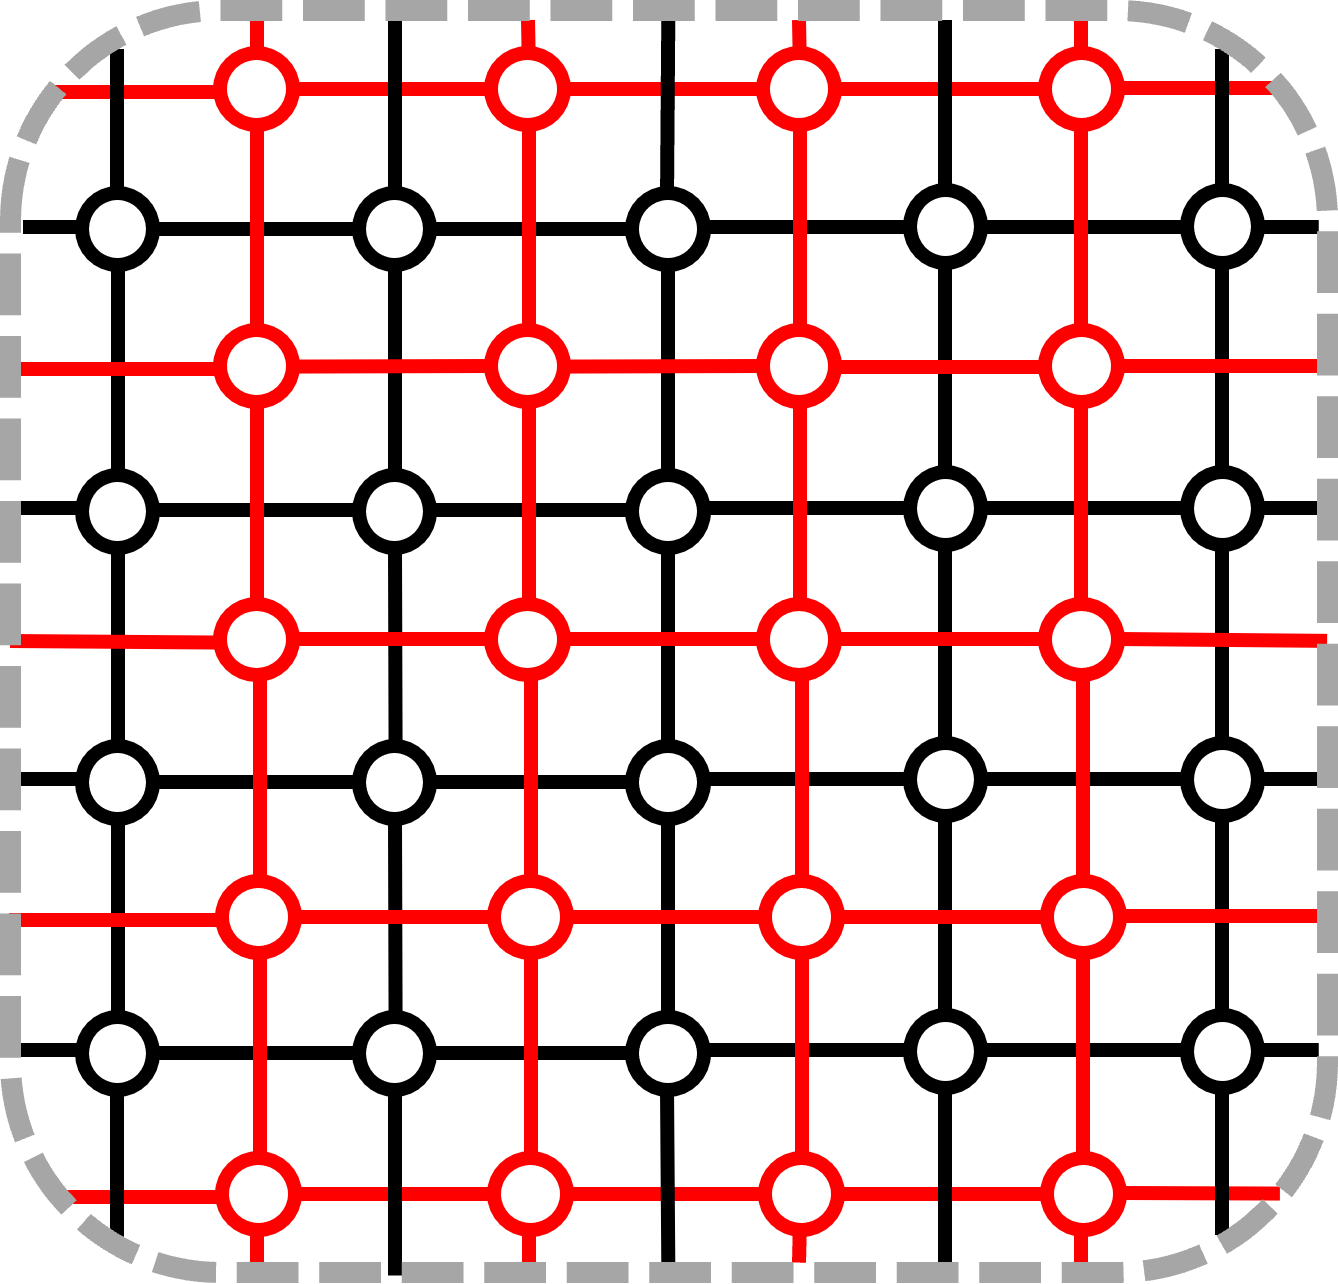
\includegraphics[scale=0.6]{drawings/dualGraph.png}
		\caption{An example snippet of the primal graph $\ints^2$ shown in black and the dual graph$(\ints^2)^*$  in red.}
		\label{fig:dualGraph}
	\end{figure}

	Thus, we can create a mapping from the open and closed edges of $\ints^2$ to the dual graph, where the edge in the dual is open if and only if the intersecting edge in $\ints^2$ is closed, and vice versa.

	Then we notice that if there exists a cycle of open edges in the dual graph enclosing the origin then the size of the open cluster at the origin is finite. 
	\begin{lemma}\label{originloop}
		$|C| < \infty$ if and only if there exists a cycle of open edges in $(\ints^2)^*$  enclosing the origin
	\end{lemma}
	\begin{proof}
		{Thinking visually since there is a ring of open edges in the dual, the open edges from the origin in the original graph cannot extend beyond this ring. A more formal pure graph theory proof can be made but is omitted here.}
	\end{proof}
	Let $X_n = \{$There is a length n cycle of open edges in $\ztwodual$ which surrounds the origin\}
	Then using Lemma~\ref{originloop} we see
	$$\prob(|C| < \infty) = \prob\left(\bigcup_{n=4}^\infty \prob(X_n)\right) \leq \sum_{n=4}^\infty \prob(X_n) \leq \sum_{n=4}^\infty n \cdot 4(3^{n-1})q^n$$
	Where in the last summation we get $4(3^{n-1})q^n$ as before by counting the number of possible edges a self avoiding walk can take then multiplying by the probability this path is open in the dual graph. 
	We multiply this term by $n$ since we know for every cycle around the origin in the dual there is some smallest $i \in \mathbb{N}$ for which the cycle crosses the edge $\{i,i-1\}$, i.e. the positive x-axis. 
	Then we can translate this cycle left and right along the `x-axis', this gives up to $n$ cycles enclosing the origin in the dual graph.


	This sum is finite when $q<1/3$, which is when $p>2/3$. 
	We can make the sum arbitrarily small when $p \rightarrow 1$, when the sum is smaller than 1 this implies $\theta(p) > 0$.
	Taking the value $p=0.9$ for example, we can calculate that the sum converges to 
	$$\sum_{n=4}^\infty n \cdot 4(3^{n-1})(1-0.9)^n = 0.0683265$$
	Thus $\theta(0.9) > 0$.

\end{proof}
Hence, the critical value $p_c(2) \in (\frac{1}{3},\frac{9}{10})$




\subsection {Existence of a critical value on \texorpdfstring{$\ints^d$}{ Zd}}
We can easily derive the result that $p_c(d)\in (0,1)$ from the previous section. 
We notice that for all $d\geq 2$ we can extract $\ints^d$ from $\ints^{d+1}$ by simply ignoring the extra edges and their states.
Thus, if there exists an infinite open cluster in $\ints^d$ this would also imply there is one in $\ints^{d+1}$.
Since we have just shown $p_c(2) \in (0,1)$ then we must also have $p_c(d) \in (0,1)$ for all d. In fact by this argument it is clear we have for $d \geq 1$ that,
$$p_c(d) \geq  p_c(d+1) $$
Since, if we couple the configurations of each lattice as mentioned by embedding $\ints^d$ into $\ints^{d+1}$ at the origin. Then as the value of $p$ increases the origin lies in an infinite open cluster of $\ints^{d+1}$ at worst at the same value of $p$ for which the origin lies in an infinite open cluster of $\ints^d$.

\section{Harris-Kesten Theorem} \label{HarrisKesten}
An important result in percolation theory is that the critical value for the square lattice is $\frac{1}{2}$. 
This result came in two parts, firstly Harris \cite{harris_1960} showed that $p_c(2) \geq \frac{1}{2}$ in 1960.
Then 20 years later Kesten \cite{kesten1980critical} proved $p_c(2) \leq \frac{1}{2}$, these proofs combined resulted in the following theorem.

\begin{theorem}[Harris-Kesten theorem]
	The critical value on $\ints^2$,  $p_c(2) =  \frac{1}{2}$.
\end{theorem}
The aim of this section is to construct a proof of this theorem. We largely follow the proofs and methods of \cite{bollobas2006short}, which in turn is largely based on the proofs by Russo, Seymour and Welsh.
To do this we first introduce some more foundational results.

\subsection{Some preliminary results}
Recall from earlier the definition of an increasing event.
\begin{definition}[Increasing Event]
	An event $ A \subseteq \Omega$ is increasing if when $\omega \in A$ and
	$$\forall e \in E(\ints^d) \text{, } \omega_e = 1 \implies \omega'_e = 1$$
	Then $\omega' \in A$. \\
\end{definition}

We now introduce an important result, known as Harris' Inequality, which tells us that the probability of increasing events are positively correlated, we follow the proof for Harris' Inequality given by \cite{duminil2018introduction}.
\begin{theorem}[Harris' Inequality] \label{harrisLemma}
If $A, B \subseteq \Omega$ are increasing events then 
$$\mathbb{P}(A \cap B) \geq \mathbb{P}(A)\mathbb{P}(B)$$
This is a specific case of a more general inequality, the FKG inequality.
If $f$ and $g$ are two bounded increasing functions then
$$ \mathbb{E}_p(fg) \geq \mathbb{E}_p(f)\mathbb{E}_p(g)$$
\end{theorem}
\begin{proof}
	% Suppose some increasing events $A,B \subseteq \Omega$ which only depend on the states of a finite number of edges.
	% Say these edges are $e_1, e_2, ... , e_n$.
	% We work by induction on the size of $n$.\\
	% Consider when $n = 1$, then both $A$ and $B$ just depend on the state of $e_1$. 
	% As both $A$ and $B$ are increasing, they must occur when $e_1$ is open since an increasing event cannot depend on edges being closed.
	% $$\mathbb{P}(A \cap B) =\prob(\omega_{e_1} = 1)= p \geq p^2 = \prob(\omega_{e_1} = 1)^2= \mathbb{P}(A)\mathbb{P}(B)$$
	% Since $p \in [0,1]$. So the theorem holds when $n=1$.\\
	
	% % \\If $A$ and $B$ occur when $e_1$ is closed then similarly to above we get.
	% % $$\mathbb{P}(A \cap B) = q \geq q^2 = \mathbb{P}(A)\mathbb{P}(B)$$
	% % Again since $q \in [0,1]$. So the theorem holds.
	% % Finally, if one of $A$ and $B$ occur when $e_1$ is open and the other when it is closed then.
	
	% Now suppose the theorem holds for $n=k$ and consider when $A$ and $B$ depend on the states of edges $e_1, e_2, ... , e_k,e_{k+1}$.
	% Let $A = A_0 \cup A_1$ where:
	% $$A_i =\{\omega \setminus (e_{k+1},\omega_{e_{k+1}}):\omega \in A\text{, }\omega_{k+1} = i\} $$
	% Similarly let $B = B_0 \cup B_1$ where the $B_i$  are defined in the same way as above.
	

	We show that the FKG inequality holds, since we can easily derive Harris' inequality by setting $f$ and $g$ to be indicator functions of the increasing events $A$ and $B$.
	We first show the result holds for increasing functions which depend on a finite number of edges, then we see how this restriction can be removed using the Martingale convergence theorem.


	Working by induction on the number of edges that the functions $f$ and $g$ depend on, we label the edges in $E = \{e_i : i \geq 1 \text{, } e_i \in E\}$.
	We also shorten our notation for the state of a given edge $\omega_{e_i} = \omega_i$ for readability during this proof.
	

	In the base case $n = 1$ we suppose $f$ and $g$ depend solely on $\omega_1$.
	Note that we can just show the inequality holds when we assume $f(0) = g(0) = 0$ since additional constants in $f$ and $g$ will not affect the inequality. 
	Since $f$ and $g$ are increasing we know that $f(1) \geq 0$ and $g(1) \geq 0$.
	So we find by the definition of expectation 

	$$\expp(fg) - \expp(f)\expp(g) = (p \cdot f(1)g(1) + q \cdot  0) - (p \cdot f(1) + q \cdot 0)(p \cdot g(1) + q \cdot 0) $$
	
	Then simplifying by removing terms multiplied by zero
	$$\expp(fg) - \expp(f)\expp(g) = pf(1)g(1) - p^2f(1)g(1) \geq 0$$
	Since $p\geq 0$, $f(1)\geq 0$ and $g(1) \geq 0$.
	So the result holds for $n=1$.


	Now assuming as our inductive hypothesis that the inequality holds for functions dependent on $n = k$ edges.
	We consider when $ n = k+1$.
	We fix the state of the first k edges, $\omega_1,...,\omega_k$, and condition on them since we aim to use the tower law for expectation later.
	Then,
	$$\expp(fg|\omega_1,...,\omega_k) = p f(\omega_1,...,\omega_k,1)g(\omega_1,...,\omega_k,1)
	+ qf(\omega_1,...,\omega_k,0)g(\omega_1,...,\omega_k,0)$$
	Where the functions $f(\omega_1,...,\omega_k,1)$ and $g(\omega_1,...,\omega_k,1)$ now depend only on the edge $\omega_{k+1}$
	Then letting $ \mathbb{P}_{\omega_{k+1}}$ be the law (distribution) of $\omega_{k+1}$ and similarly $\mathbb{E}_{\omega_{k+1}}$.
	We see that 
	\begin{align*}
		\expp(fg|\omega_1,...,\omega_k) &= p f(\omega_1,...,\omega_k,1)g(\omega_1,...,\omega_k,1)\\
	&+ qf(\omega_1,...,\omega_k,0)g(\omega_1,...,\omega_k,0)\\
	&= \mathbb{E}_{\omega_{k+1}}(f(\omega_1,...,\omega_k,\cdot)g(\omega_1,...,\omega_k,\cdot))\\
	\end{align*}

	Then applying our inductive hypothesis.
	$$\mathbb{E}_{\omega_{k+1}}(f(\omega_1,...,\omega_k,\cdot)g(\omega_1,...,\omega_k,\cdot))
	\geq \mathbb{E}_{\omega_{k+1}}(f(\omega_1,...,\omega_k,\cdot))\mathbb{E}_{\omega_{k+1}}(g(\omega_1,...,\omega_k,\cdot))$$
	Which means
	$$ \mathbb{E}_p(fg|\omega_1,...,\omega_k) \geq \mathbb{E}_p(f|\omega_1,...,\omega_k)\mathbb{E}_p(g|\omega_1,...,\omega_k)$$
	So applying the tower law of expectation 
	\begin{align*}
		\expp(fg) &= \expp(\expp(fg|\omega_1,...,\omega_k))\\
		&\geq \expp(\expp(f|\omega_1,...,\omega_k)\expp(g|\omega_1,...,\omega_k))\\
		&\geq \expp(\expp(f|\omega_1,...,\omega_k))\expp(\expp(g|\omega_1,...,\omega_k))\\
		&= \expp(f)\expp(g)
	\end{align*}
	So we have shown the result for all increasing functions which depend on a finite number of edges.
	Now to extend this to arbitrary bounded increasing functions we consider the martingale convergence theorem.
	For our bounded increasing functions $f$ and $g$ we define:
	\begin{align*}
		f_n &:= \expp(f | \omega_1,...,\omega_n)\\
		g_n &:= \expp(g | \omega_1,...,\omega_n)
	\end{align*}
	We note that $(f_n)$ and $(g_n)$ form martingales due to the tower law of expectation.
	Then since we assumed $f$ and $g$ are bounded we can apply the martingale convergence theorem to see that $f_n$ converges to $f$  as $n \rightarrow \infty$ and similarly $g_n$ converges to $g$.
	We do not give a rigorous proof of this here, but the reader may wish to seek further information on Doob's martingale convergence theorem from \cite{williams_1991}.
	

\end{proof}
We also note a useful rearrangement of Harris' Inequality which captures the idea that the events $A$ and $B$ are positively correlated.
\begin{corollary}
	If $A, B \subseteq \Omega$ are increasing events then 
	$$\prob(A|B) \geq \prob(A)$$
	Intuitively this makes sense, the probability A occurs increases when we know more edges are open, and knowing B has occurred tells us about open edges.
\end{corollary}

We now prove a useful inequality for events that occur disjointly, first we define what we mean for events to occur disjointly.
\begin{definition}[Disjoint realisation of events]
	Let $A$ and $B$ be events. For a configuration $\omega \in A$, there is some witness set $I \subset E$ for $\omega$ such that for any other configuration $\omega'$ which satisfies:
	$$\forall e \in I \text{, } \omega_e = \omega'_e$$
	Then $\omega' \in A$, in essence the states of edges in $I$ tell us the event $A$ has occurred in $\omega$.\\
	We say the events $A$ and $B$ occur disjointly in $\omega$, denoted $A \circ B$, if there exists disjoint witnesses $I$ and $J$ for $A$ and $B$ respectively. I.e. $I \cap J = \emptyset$

\end{definition}

This concept is different to the intersection of events, since intuitively the edges on which each event occurs cannot overlap.
For example given some $n\times n$ box of $\ints^2$, the event there is an open crossing from top to bottom and the event there is an open crossing left to right cannot occur disjointly. Since the open paths will cross at some point.
We now state the inequality we aim to prove.
\begin{theorem}[BK inequality]
	If $A, B \subseteq \Omega$ are increasing events then
	$$\prob(A \circ B) \leq \prob(A)\prob(B)$$
\end{theorem}
\begin{proof}
	We follow the proof given by \cite{bollo2006} which is easier than the original.
	We work by induction on the size of the edge set $E$ which we denote by $n$, remembering the sample space $\Omega = \{0,1\}^E$.
	When $n = 0$ the inequality holds trivially.
	Supposing as our inductive hypothesis that the inequality holds when the edge set has size less than $n$.
	We show it also holds when $E$ has size n.
	First we define for any subset $D \subseteq \{0,1\}^E$:
	\begin{align*}
		D_0 &= \{(\omega_1,...,\omega_{n-1}) : (\omega_1,...,\omega_{n-1}, 0 ) \in D\}\\
		D_1 &= \{(\omega_1,...,\omega_{n-1}) : (\omega_1,...,\omega_{n-1}, 1 ) \in D\}
	\end{align*}
	Then we can decompose the probability of D since the states of edges are independent.
	$$\prob(D) = p\prob(D_1) + q\prob(D_0)$$
	Now for our increasing $A,B \subseteq \{0,1\}^E$, define $C = A \circ B$, we now see that 
	$$C_0 = A_0 \circ B_0$$
	$$C_1 = (A_1 \circ B_0) \cup (A_0 \circ B_1)$$
	Applying our assumption that $A$ and $B$ are increasing its clear that $A_0 \subseteq A_1$ and $B_0 \subseteq B_1$.
	Thus we find,
	$$C_0 = A_0 \circ B_0 \subseteq (A_1 \circ B_0) \cap (A_0 \circ B_1)$$
	$$C_1 = (A_1 \circ B_0) \cup (A_0 \circ B_1) \subseteq A_1 \circ B_1$$
	Using this decomposition in conjunction with our inductive hypothesis we find 
	$$\prob(C_0) = \prob(A_0 \circ B_0) \leq \prob(A_0)\prob(B_0)$$
	$$\prob(C_1) \leq \prob(A_1 \circ B_1) = \prob(A_1)\prob(B_1)$$
	Now we can also get by adding the probabilities of $C_0$ and $C_1$ that 
	\begin{align*}
		\prob(C_0) + \prob(C_1) &\leq \prob((A_1 \circ B_0) \cap (A_0 \circ B_1)) + \prob((A_1 \circ B_0) \cup (A_0 \circ B_1))\\
								&= \prob(A_0 \circ B_1) + \prob(A_1 \circ B_0)\\
								&\leq \prob(A_0)\prob(B_1) + \prob(A_1)\prob(B_0)
	\end{align*}
	The next step is to combine these by finding 
	$$(1-p)^2\prob(C_0) + p^2\prob(C_1) + p(1-p)(\prob(C_0) + \prob(C_1))$$
	$$=((1-p)^2 + p(1-p))\prob(C_0) + (p^2 + p(1-p))\prob(C_1) = (1-p)\prob(C_0) + p\prob(C_1)$$
	Then looking at the right-hand sides
	\begin{align*}
		(1-p)\prob(C_0) + p\prob(C_1) \leq& (1-p)^2[\prob(A_0)\prob(B_0)]\\
		&+ p^2[\prob(A_1)\prob(B_1)]\\
		& +p(1-p)[\prob(A_0)\prob(B_1) + \prob(A_1)\prob(B_0)]
	\end{align*}
	Which simplifies to 
	$$(1-p)\prob(C_0) + p\prob(C_1) \leq [p\prob(A_1) + (1-p)\prob(A_0)][p\prob(B_1) + (1-p)\prob(B_0)]$$
	Then using $\prob(D) = p\prob(D_1) + (1-p)\prob(D_0)$ we see that
	$$\prob(A \circ B) = \prob(C) \leq \prob(A)\prob(B)$$

\end{proof}

% {\color{red} MIGHT NOT BE NEEDED WITH RSW PROOF.
% Using the BK inequality we can now show a useful inequality more specific to percolation.
% \begin{corollary}
% 	For a finite subset $S \subset \ints^d$ which contains the origin, and some $x \notin S$, 
% 	$$\prob(0 \longleftrightarrow x) \sum_{y\in \partial S} \prob({0\stackrel{S}{\longleftrightarrow}y})\prob(y \longleftrightarrow x)$$
% 	Where $0\stackrel{S}{\longleftrightarrow}y$ occurs if $0$ is connected to $y$ by open edges in $S$. If no set S is given we allow any open edges.
% 	Also, $\partial S$ denotes the vertex boundary of S, i.e. $\forall s \in \partial S$, the neighbourhood of s contains some $x \in \ints^d \setminus S$
% \end{corollary}
% \begin{proof}
% 	{\color{red} todo}
% 	Work on an n by n box.
% \end{proof}
% }
\subsection{Crossing rectangles}

We now introduce some notation to allow us to discuss rectangles and their crossings in a succinct manner.
\begin{definition}
	Let $R = [a,b]\times[c, d]$ for integers $a<b$, $c<d$ be a rectangle, we identify this rectangle with a subgraph of $\ints^2$ which includes all vertices and edges on the boundary and inside. Let $k = b-a$ and $l = d-c$, then we say that R is a $k$ by $l$ rectangle.
	
	We now let $H(R)$ denote the event that there is a horizontal open crossing of R, i.e. a path from the left boundary of R to the right only using open edges. Similarly, we define $V(R)$ to be the event that there is a vertical open crossing of R. 
\end{definition}

We note from this definition that if $R$ and $R'$ are distinct rectangles, which includes their boundaries being distinct. Then the events $H(R),V(R)$ are independent of $H(R'),V(R')$.

It is also useful to specify how the subgraph identified with a rectangle is related to the dual graph, $\ztwodual$.
\begin{definition}
	The (horizontal) dual of a rectangle $R = [a,b]\times[c,d]$ in $\ints^2$ is the rectangle $R^h = [a+1/2,b-1/2]\times[c-1/2,d+1/2]$ in $\ztwodual$. As a reminder an edge in the dual is open if and only if the edges it intersects in the primal lattice is closed.
	Let $V^*(R^h)$ be the event there is a vertical crossing of $R^h$ in the dual graph by open edges.
\end{definition}

\begin{figure}
	\centering
	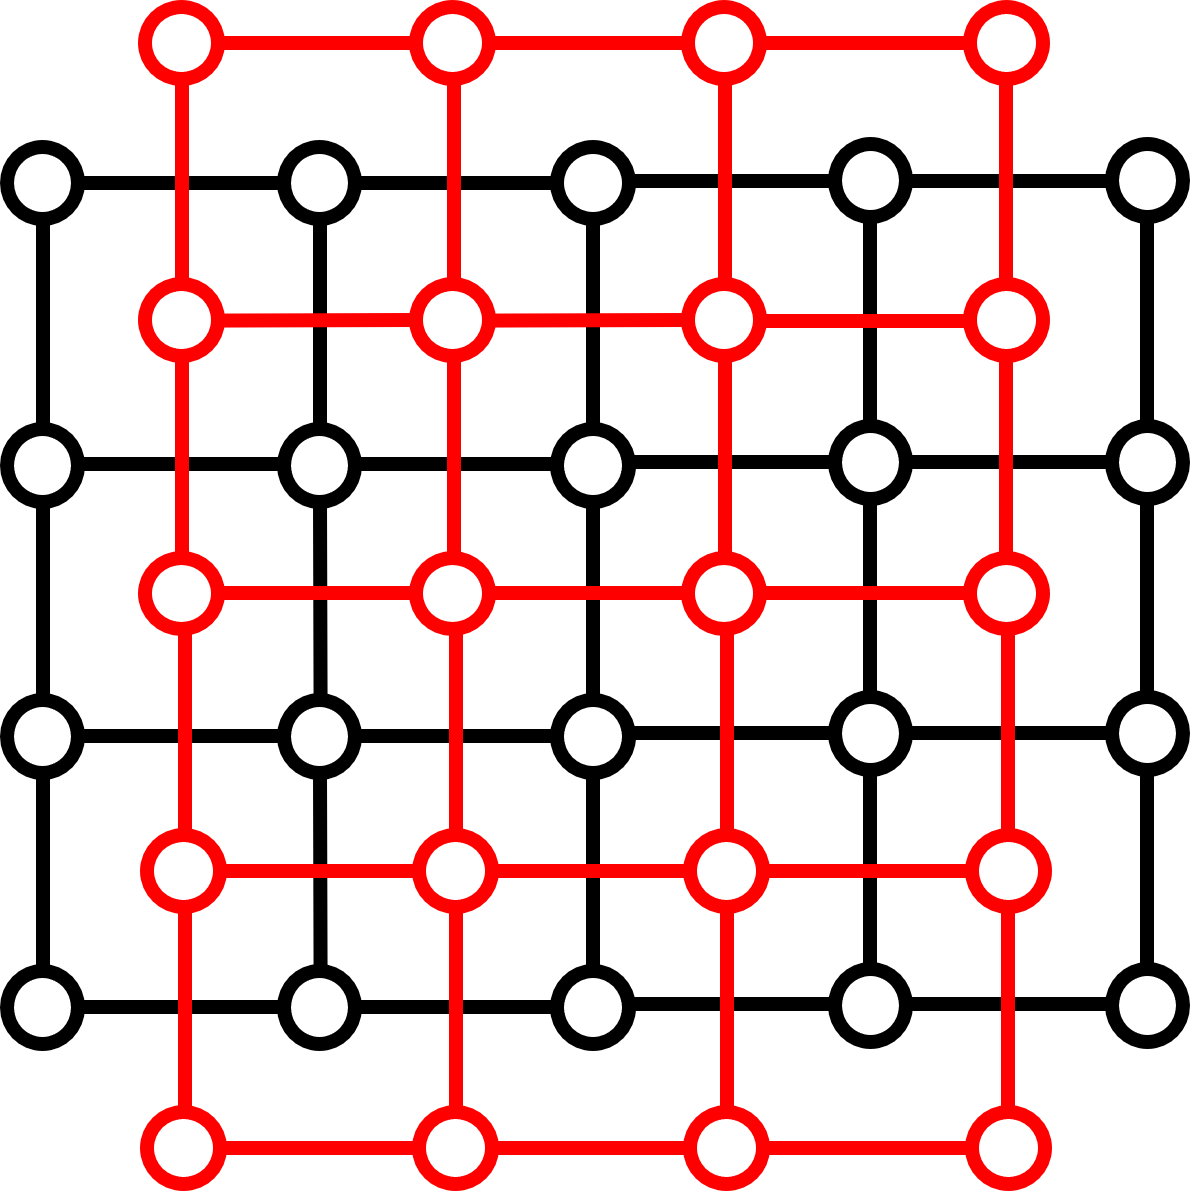
\includegraphics[scale=0.6]{drawings/RectangleDual2.png}
	\caption{An example 5 by 4 rectangle $R$ shown in black and the dual $R^h$ in red.}
	\label{fig:rectangle}
\end{figure}

We now prove an important result similar to that of Lemma~\ref*{originloop}, for rectangles. Relating the horizontal crossings in primal rectangles to vertical crossings in their duals.

\begin{lemma}\label{rectangleProof}
	Let $R$ be a rectangle in $\ints^2$. For any configuration $\omega$ of $\ints^2$, exactly one of the events $H(R)$ and $V^*(R^h)$ holds.
\end{lemma}

\begin{proof}
	Without loss of generality we scale the lattice to avoid working with fractions. Let the lattice $L = (0,2) + 4\ints^2$, and hence its dual $L^* = (2,0)+4\ints^2$. Then let R be a $k$ by $l$ rectangle on $L$ with vertex set $\{(4i,4j+2): 0 \leq i \leq k \text{, } 0 \leq j \leq l-1 \}$, and thus we have that $R^h$ has vertex set $\{(4i+2,4j): 0 \leq i \leq k-1 \text{, } 0 \leq j \leq l \}$. Suppose some percolation configuration of $\ints^2$ and let G be the graph induced by the open edges of $R$, similarly let the open edges of $R^h$ induce the graph $G^h$. Now it suffices to show that either $G$ contains a left-right path or $G^h$ contains a top-bottom path, but not both. If we wish to show that $G$ has a left-right, i.e. a path from $(0,4m+2)$ to $(4k,4n+2)$ for some $m,n \in \mathbb{N}$, then we can assume without loss of generality that $G$ contains all $2(l-1)$ edges on its left and right most sides. We make a similar assumption that $G^h$ has all $2(k-1)$ on its top and bottom. This means we only have to consider one vertex each of the sides of the rectangles.

	We now construct a third graph, $M$, which lies between $G$ and $G^h$. Let $R_{odd}$ be a $2k\times 2l$ rectangle with vertex set $\{(2i+1,2j+1): 0 \leq i \leq 2k-1 \text{, } 0 \leq j \leq 2l-1 \}$, then let M be the subgraph of $R_{odd}$ which just contains edges that do not intersect edges of $G$ nor $G^h$. We direct all the edges of $M$ such that edges of $G$ lie on the right and $G^h$ lie on the left. It is evident that this results in all vertices of M having one edge in and one edge out, except for 4 vertices of degree one which lie in the ``corners'' of the rectangle, label them counter-clockwise $x,y,z,w$ as in Figure~\ref*{fig:rectangleProof}. Clearly due to the way we previously oriented the edges of $M$, $x$ and $z$ have one out edge, $y$ and $w$ have one in edge. Hence, the component of $M$ which $x$ lies in must be a path, say $P$, which ends at either $y$ or $w$. In the case where $P$ ends at $y$, then we have that the subgraph of $G^h$ to the left of $P$ must be connected from the top to the bottom. Thus, by basic graph theory this subgraph must contain a top-bottom path. If we are in the case where $P$ ends at $w$ then we must have the subgraph of $G$ to the right of $P$ is connected from left to right, thus meaning it admits a left-right path. Clearly then at least one of $H(R)$ and $V^*(R^h)$ occurs.
	\begin{figure}
		\centering
		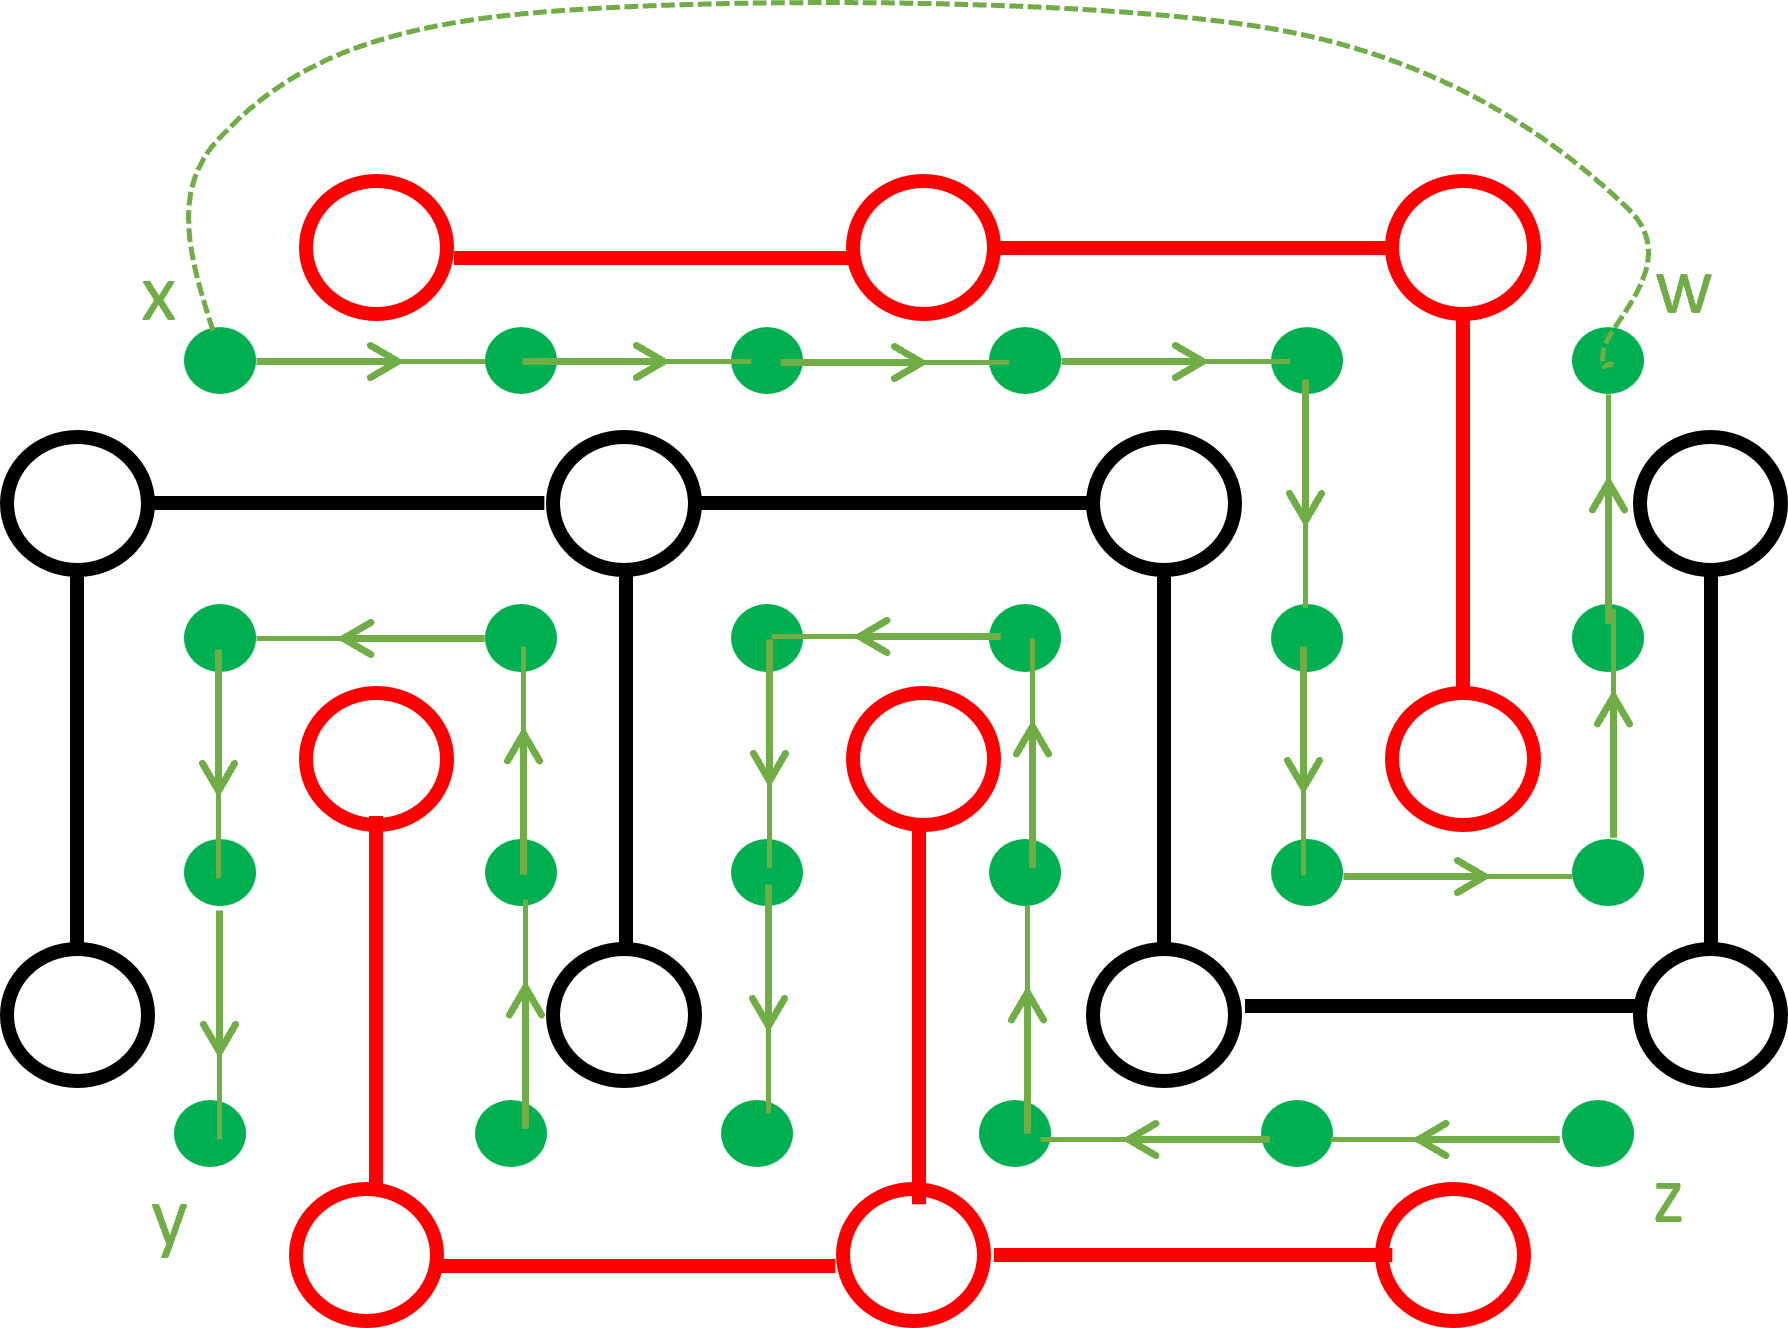
\includegraphics[scale=0.6]{drawings/rectanglesproof.png}
		\caption{An example with $G$ in black, $G^h$ in red and $M$ in green. The dashed green line shows the Jordan Curve construction.}
		\label{fig:rectangleProof}
	\end{figure}
	To show that exactly one  $H(R)$ and $V^*(R^h)$ occurs we utilise the Jordan Curve Theorem. A brief summary of this result is, given a non-self-intersecting continuous closed loop in the plane, $J$, called a Jordan Curve, then $J$ divides the plane into two distinct regions, an inside and an outside whose boundary is $J$. We refer the reader to \cite{kosniowski_1980} for a proof of the Jordan Curve Theorem. If the path $P$ runs from $x$ to $w$ then $P$ can be extended to a Jordan curve $J$ by simply adding a curve from $w$ to $x$ over the top of all the vertices of $R^h$. This results in all the vertices on the top of $R^h$ lying inside the Jordan curve and the vertices at the bottom of $R^h$ lie on the outside of the curve. Hence, any top-bottom path in $G^h$ must cross $J$ which means it crosses an edge of $M$, but this contradicts the definition of the edges of $M$. So only $H(R)$ occurs.
	Similarly, in the case that $P$ ends at $y$, we form a Jordan curve by connecting $x$ to $y$ on the left of the vertices on the left side of $G$. Then by an analogous argument to before, we cannot have a left-right path in $G$ since the left and right sides lie in the interior and exterior of the Jordan curve respectively. Hence, only $V^*(R^h)$ occurs in this case.
\end{proof}

We note that the edges of $L^*$ above are open with probability $1-p$, and so we can form some useful results for rectangles in $\ints^2$ directly from this lemma.

\begin{corollary}
	If $R$ is a $k$ by $l-1$ rectangle in $\ints^2$ and $R'$ is a $k-1$ by $l$ rectangle. Then,
	$$\prob(H(R))+\mathbb{P}_{1-p}(V(R')) = 1 $$
\end{corollary}

Further to this, if $k = l = n+1$ for some $n$, then $R'$ is simply a 90-degree rotation of $R$. Hence, $\prob(H(R)) = \mathbb{P}_{1-p}(V(R')$. From this we find the key statement due to the self-duality of $\ints^2$ we discussed in Section~\ref*{critvalZ2}.

\begin{corollary}\label{squareGEQhalf}
	If $R$ is an n+1 by n rectangle then $\mathbb{P}_{1/2}(H(R)) = 1/2$. So for $n$ sided square $S$, which is just defined as an $n$ by $n$ rectangle. We must have,
	$$\mathbb{P}_{1/2}(H(S))=\mathbb{P}_{1/2}(V(S)) \geq 1/2$$
\end{corollary}

While it might now feel intuitively obvious that $p_c(2) \geq 1/2$, and certainly Corollary~\ref*{squareGEQhalf} is essential in the reasoning for this, we are yet to prove it rigorously.

\subsection{Harris' Theorem}

In order to make this idea rigorous, we now aim to show that $\theta(1/2) = 0$. This is Harris' Theorem, although the method we use will be different to Harris' original as previously mentioned, we follow the ideas of Russo, Seymour and Welsh.

\begin{lemma}\label{mby2nLemma}
	Let $R = [0,m]\times[0,2n]$ be an $m$ by $2n$ rectangle with $m\geq n$. Let $X(R)$ be the event that there are paths $P_1$ and $P_2$ of open edges, where $P_1$ crosses the square $S = [0,n]\times[0,n]$ from top to bottom, and $P_2$ lies inside $R$ and joins some vertex on $P_1$ to some vertex on the right side of $R$. Then, 
	$$\prob(X(R))\geq \frac{1}{2}\prob(H(R))\prob(V(S))$$
\end{lemma}
\begin{proof}
	We first suppose that $V(S)$ holds, so there is a path $P$ of open edges crossing the square top to bottom. This path separates $S$ into two regions, by the Jordan Curve Theorem. In fact, we choose the left most path $P$, call it $LV(S)$, and we note that the event $\{LV(S) = P_1\}$ does not depend on any edges to the right of $P_1$. We can do this due to our proof of Lemma~\ref{rectangleProof}, if $V(S)$ holds we have a path from $x$ to $y$ in $M$, and $LV(S)$ is directly adjacent on the left of the path(when viewed from the edge direction) from $x$ to $y$, in doing so we only needed to look at the edges to the left of $LV(S)$.

	\begin{figure}
		\centering
		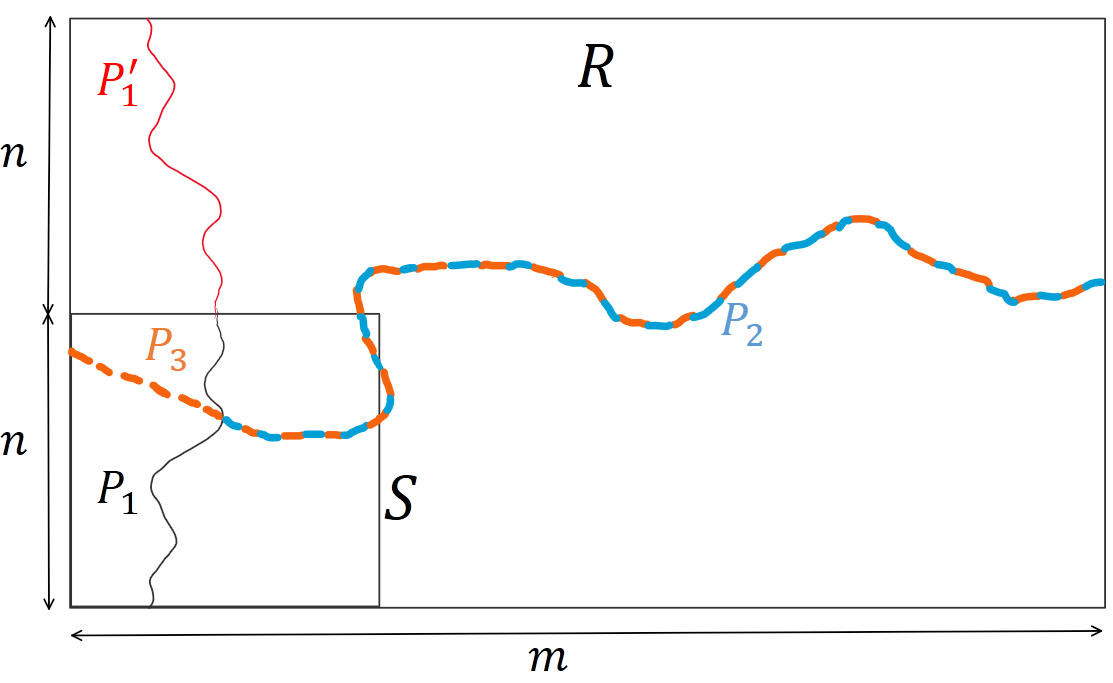
\includegraphics[scale=0.48]{drawings/2nbymRectangle.png}
		\caption{An example m by 2n rectangle R, where $P_3$ crosses $P_1$ and thus the event $X(R)$ has occurred.}
		\label{fig:2nbymProof}
	\end{figure}

	Now let $P$ be the path constructed by joining $P_1$ to its reflection $P_1'$ in the line $y=n$, note $P$ may not necessarily be open. Then $P$ crosses the left $[0,n] \times [0,2n]$ section of $R$ top to bottom. By definition, we know with probability $\prob(H(R))$ there is an open path $P_3$ crossing $R$ left to right. We know this path $P_3$ must cross $P$ at some vertex. Due to symmetry by which we constructed $P$, we know the probability that $P_3$ crosses $P$ at a vertex in $P_1$ (the bottom half of P) is at least $\prob(H(R))/2$. Now let $Y(P_1)$ be the event there is an open path $P_2$ from the RHS of $R$ to some vertex of $P_1$, then clearly $Y(P_1)$ must occur with probability at least $\prob(H(R))/2$ too. We note that the event $Y(P_1)$ only depends on the edges to the right of $P_1$. So since the event $\{LV(S) = P_1\}$ does not depend on any edges to the right of $P_1$ as previously mentioned, $Y(P_1)$ and $\{LV(S) = P_1\}$ are independent. So we have:
	$$\prob(Y(P_1) \, | \, LV(S) = P_1) = \prob(Y(P_1)) \geq \prob(H(R))/2 $$
	Furthermore we can see that $Y(P_1)$ and $\{LV(S) = P_1\}$ occurring implies that $X(R)$ has occurred. So, it is clear that:
	$$\prob(X(R) \, | \, LV(S) = P_1) \geq \prob(H(R))/2 $$
	Finally we that the event there is a vertical crossing of $S$, $V(S)$, is the disjoint union of the events ${LV(S) = P_1}$ for all $P_1$ in $S$. So, we get that:
	$$\prob(X(R) \, | \, V(S)) \geq \prob(H(R))/2 $$
	Then by simple rearrangement we get the required result.

\end{proof}

We now prove an important corollary of the above lemma which bounds below the probability of a horizontal crossing in specific shapes of rectangles. We follow the method used in \cite{bollobas2006short} by Bollob\'as and Riordan which differs from the original methods of Russo, Seymour and Welsh, which can be found in \cite{grimmett1999percolation}.

\begin{corollary}\label{rectangleBound}
	Let $\rho >1$ be a fixed integer. Then there is a constant $c_2(\rho) > 0$ which is only dependent on $\rho$ such that, for any $2\rho n$ by $2n$ rectangle $R$ we have $\mathbb{P}_{1/2}(H(R)) \geq c_2(\rho)$
\end{corollary}

\begin{proof}
	Let $h_{m,n} = \mathbb{P}_{1/2}(R_{m,n})$ where $R_{m,n}$ is an m by n rectangle. We aim to show that for $m>n$ we have
	\[
		h_{2m-n,2n} \geq \frac{h_{m,2n}^2}{2^5} \tag{$\star$}
	\]
	
	Since then we can iteratively apply the inequality using ${h_{2n,2n} \geq 1/2}$ from Corollary~\ref*{squareGEQhalf} to begin, repeating until we reach $h_{2\rho n,2n}$. For example the first step would be:
	$$h_{3n,2n} =h_{2(2n) -n,2n} \geq \frac{h_{2n,2n}}{2^5} \geq \frac{1/2}{2^5} = 2^{-6}$$

	So in order to show $(\star)$ holds we consider intersecting rectangles $R = [0,m]\times [0,2n]$ and $R' = [n-m,n] \times [0,2n]$, in addition to the lower square $S = [0,n] \times [0,n]$ inside both.
	Let $E_1 = X(R)$ then let $E_2$ be the corresponding event reflected in the line $y=n/2$ for $R'$. Let $E_3 = H(S)$ be the event there is a horizontal crossing of S.
	Then if $E_1,E_2,E_3$ all hold we have that $H(R \cup  R')$ holds, by the fact that the horizontal crossing of $S$ must cross the two vertical crossing of $S$ which occur due to $E_1,E_2$. This is shown in Figure~\ref{fig:doubleRectangle}.
	\begin{figure}
		\centering
		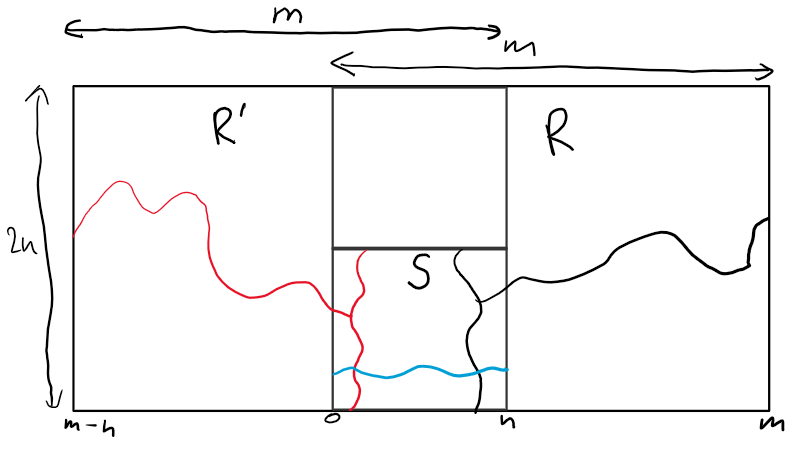
\includegraphics[scale=0.6]{drawings/doubleRectangle.png}
		\caption{An example of an overlapping $R$ and $R'$, with the edges of the event $E_1$ in black, $E_2$ in red and $E_3$ in blue.}
		\label{fig:doubleRectangle}
	\end{figure}
	Then we note that $E_1,E_2,E_3$ are all increasing events, so we can use Harris' Inequality which gives us:
	\begin{align*}
	\prbhlf(H(R \cup R')) &\geq \prbhlf(E_1 \cap E_2\cap E_3)\\
	& \geq \prbhlf(E_1)\prbhlf(E_2)\prbhlf(E_3)\\
	& \geq \prbhlf(X(R))^2\prbhlf(H(S))
	\end{align*}
	Where the last line is a result of the symmetry of $E_1$ and $E_2$. From Corollary~\ref{squareGEQhalf} we know $\prbhlf(V(S)) =\prbhlf(H(S)) \ geq 1/2$, and using the result Lemma~\ref{mby2nLemma} we can plug into the above to get.
	\begin{align*}
		\prbhlf(H(R \cup R')) & \geq \prbhlf(X(R))^2\prbhlf(H(S)) \\
		& \geq \{2^{-1} \prbhlf (H(R)) \prbhlf (V(S))\}^2*1/2 \\
		& \geq (1/2)^2 \prbhlf(H(R))^2(1/2)^2*1/2 \\
		& = \prbhlf(H(R))^2/2^5
	\end{align*}
	This proves $(\star)$ and hence the Corollary holds. 
\end{proof}

We now need one more result before we can prove Harris' Theorem, the second Borel-Cantelli Lemma which we give without proof. 
\begin{lemma}[Second Borel-Cantelli Lemma]
	Let $(E_n)_{n=1}^\infty$ be an infinite sequence of events. If $(E_n)_{n=1}^\infty$ are all independent and $\sum_{n=1}^{\infty} \mathbb{P}(E_n) = \infty$ Then $\mathbb{P}(\text{infinitely many }E_n\text{ occur}) = 1$.
\end{lemma}

We are now in a position to prove Harris' theorem.

\begin{theorem}[Harris' theorem]
	For Bernoulli bond percolation on $\ints^2$ we have that $\theta(1/2) = 0$.
\end{theorem}

\begin{proof}
	We work by constructing a sequence of square annuli in the dual graph. The first annulus is formed by arranging four 6n by 2n rectangles around the origin such that the 2n by 2n ends of each rectangle overlap. See Figure~\ref{fig:squareAnnulus} for the arrangement, we note that the chosen direction to offset the annulus in the dual does not matter so long as it encloses the origin of the primal graph. 
	\begin{figure}
		\centering
		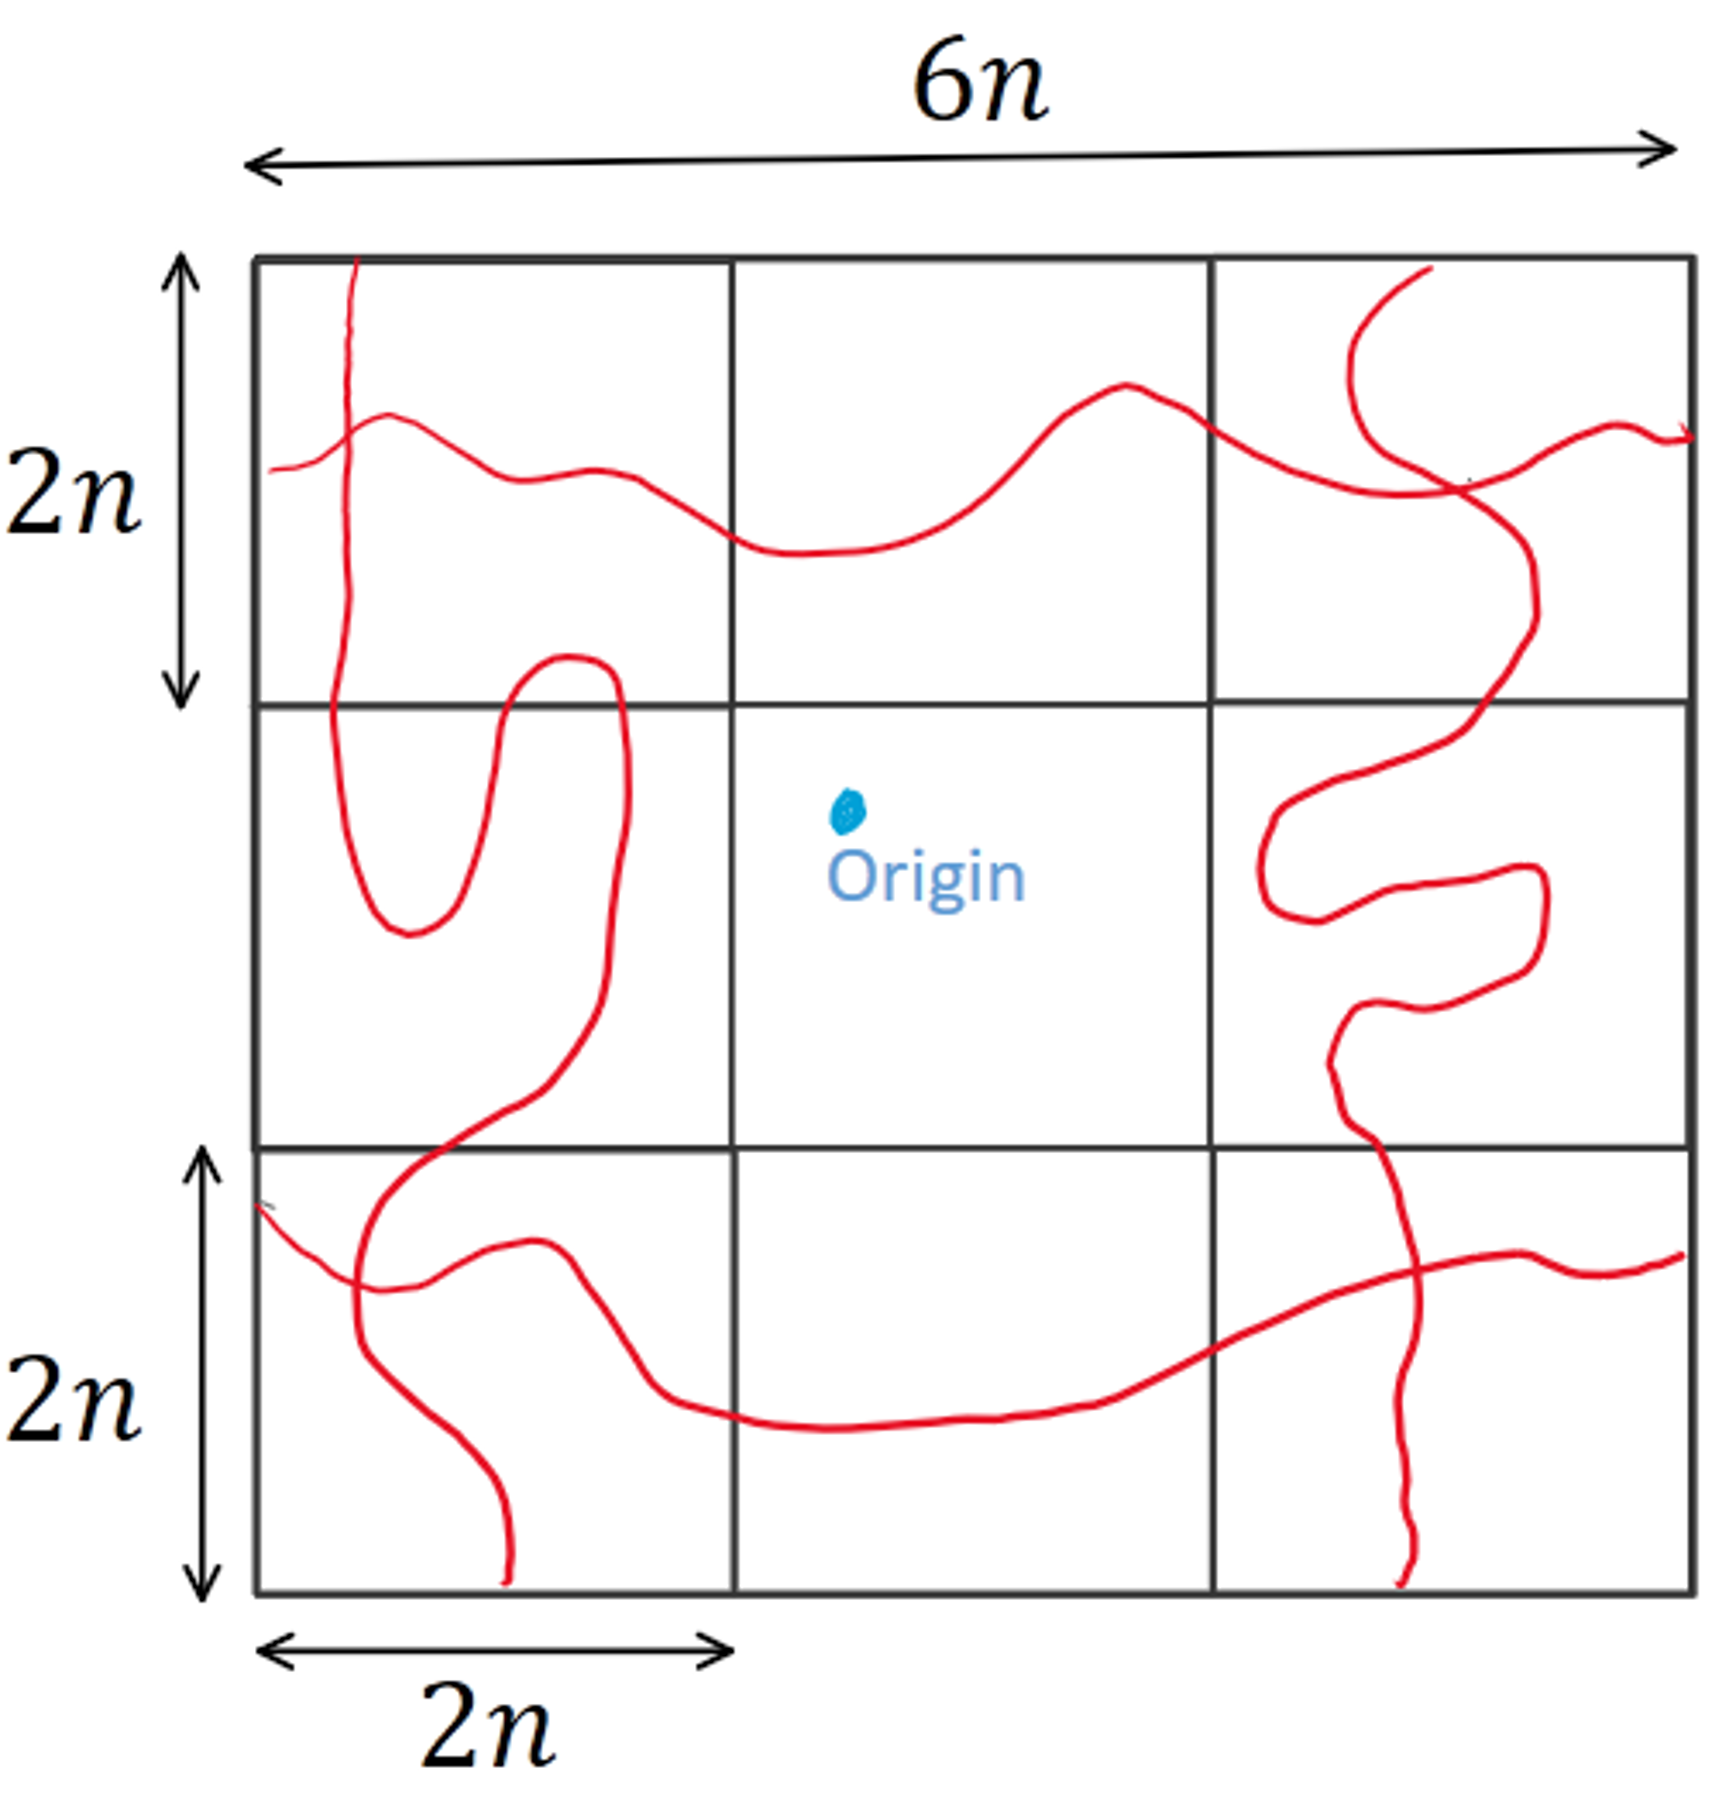
\includegraphics[scale=0.48]{drawings/squareAnnulus.png}
		\caption{An example of the first square annulus in the dual graph with the four rectangle crossings shown in red which enclose the origin.}
		\label{fig:squareAnnulus}

	\end{figure}
	Then by Corollary~\ref{rectangleBound} each rectangle has an open crossing in the long direction with probability at least $c_2(3)$, and thus all of them do with probability at least $c_2(3)^4$. When all four rectangles have an open crossing they form an open path in the dual which encloses the origin. Let $A_k$ be the square annulus in the dual graph formed by overlapping four $(2k+4)n$ by $2n$ rectangles as above. Then let $E_k$ be the event that the annulus contains an open cycle enclosing the origin. Then $\prbhlf(E_k) \geq c_2(k+2)$ by Corollary~\ref{rectangleBound}. Now since the annuli $(A_k)$ lie on disjoint regions, we have that the $(E_k)$ are all independent.
	Since $\sum_{k=1}^{\infty}\prbhlf(E_k) \geq \sum_{k=1}^{\infty}c_2(k+2)^4 = \infty$ we can apply the second Borel-Cantelli Lemma.

	$$\prbhlf(\text{infinitely many }E_k\text{ occur}) = 1$$

	Take the first $E_k$ which occurs, then the annulus $A_k$ in the dual graph contains an open cycle enclosing the origin. Thus, there cannot be an infinite cluster containing the origin in the primal graph.
\end{proof}

\subsection{Kesten's Theorem}
We now move onto proving Kesten's theorem, specifically that the percolation threshold is less than or equal to a half. In this section we again follow the definitions and methods detailed in \cite{bollobas2006short}. Firstly we introduce a powerful result due to Friedgut and Kalai \cite{friedgut1996every}.
We assume the reader has some basic group theory knowledge, although it is not critical to understanding.

\begin{definition}[Symmetric event]
	An event $\mathcal{A} \subseteq \mathcal{P}(X)$ is symmetric if there is a permutation group  $G$ acting transitively on $\mathcal{P}(X)$ which preserves $\mathcal{A}$
\end{definition}
 To explain briefly, the action of a group $G$ on a set $X$ is transitive if for all $x,y \in X$, there exists $g \in G$ such that $g \cdot  x = y$. This means G shuffles the elements of X, in essence given some $x \in X$ you can obtain any $y \in X$ by some $g \in G$. Then an event $\mathcal{A}$ being preserved under $G$ just means that if $A \in \mathcal{A}$ then there exists $g \in G$ such that $g(A) \in \mathcal{A}$. 


\begin{theorem}[Friedgut-Kalai sharp threshold theorem]\label{sharpThreshold}
	There is an absolute constant $c_1$ such that if $\mathcal{A} \subset \mathcal{P}(X)$ is a symmetric increasing event and if $\prob(\mathcal{A}) > \epsilon$ for some $0 < \epsilon < 1/2$ then, 
	$$\mathbb{P}_q(\mathcal{A}) > 1 - \epsilon$$
	whenever we have 
	$$q - p \geq c_1 \frac{log(1/(2\epsilon))}{log |X|}$$
\end{theorem}

We do not give the proof since it is too long to include within the scope of this project, but the reader is recommended to view \cite{friedgut1996every} for details. This theorem tells us all symmetric increasing events have 'sharp threshold', meaning a small increase of order $1/log|X|$ to the parameter $p$ is enough to take the probability of the event from a value close 0 to nearly 1.

Using the Friedgut-Kalai sharp threshold theorem we will now work to prove that when $p>1/2$ the probability of crossing rectangles larger than a certain size is close to 1.

\begin{lemma}\label{kesternLemma}
	Let $p >1/2$ and fix some integer $\rho >1$. Then there exists constants $\delta = \delta(p) > 0$ and $n_0 = n_0(p,\rho)$ such that when $n > n_0$ and $R_n$ is a $4\rho n$ by $4n$ rectangle on the square lattice then, $$\prob(H(R_n)) \geq 1-n^{-\delta}$$
\end{lemma}

\begin{proof}
	For the sake of simplicity, we prove the case of $\rho = 3$ since this implies the result for $\rho =2$ and these are the only cases we will later need. The other cases can be proved by an analogous argument. Let $p>1/2$, then by Corollary~\ref*{rectangleBound} with $\rho = 7$ we know there exists a constant $0<c_2<1/2$ such that for any 14n by 2n rectangle $R$, the probability of a horizontal crossing is bounded below by $c_2$, $\mathbb{P}_{1/2}(H(R)) \geq c_2$. Now we cannot directly apply the Friedgut-Kalai sharp threshold theorem since $H(R)$ is not a symmetric event, since $X$ in this case is the set of all edges in $\ints^2$. In order to get around this we introduce new symmetric events on the discrete torus. 
	\begin{definition}[Discrete Torus]
	For $n \geq 3$, the $n$ by $n$ discrete torus, $\mathbb{T}_n$, is the Cartesian product of two length n cycles. Equivalently $\mathbb{T}_n$ can be formed by identifying all pairs of vertices on $\ints^2$ whose coordinates are congruent modulo $n$. We note that $\mathbb{T}_n$ has $n^2$ vertices and $2n^2$ edges.
	\end{definition}

	\begin{figure}
		\centering
		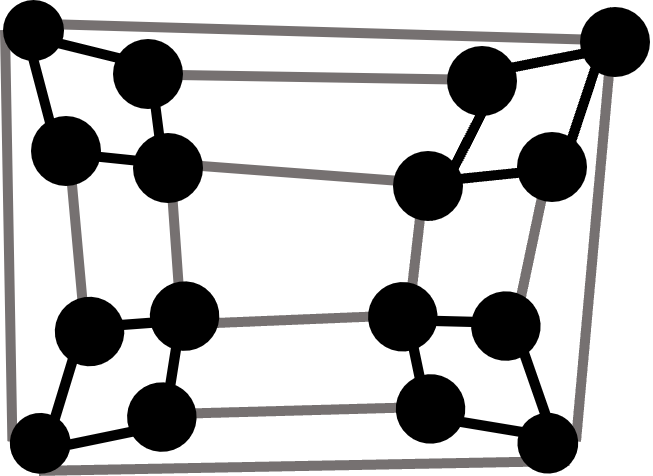
\includegraphics[scale=0.8]{drawings/torus.png}
		\caption{$\mathbb{T}_4,$ the 4 by 4 discrete torus.}
		\label{fig:torus}
	\end{figure}

	Now for $1 \leq k,l \leq n-2$, we define a $k$ by $l$ rectangle $R$ in $\mathbb{T}_n$ to be an induced subgraph in $\mathbb{T}_n$ which has an associated $k$ by $l$ rectangle $R' = [a,a+k] \times [b,b+l]$ in $\ints^2$, for some $a,b \in \ints$. Due to the restriction in size of $k$ and $l$ our rectangles in the torus never wrap around on themselves and thus always have an associated planar rectangle in $\ints^2$.
	
	We define Bernoulli bond percolation on $\mathbb{T}_n$ as you would expect, where each edge is open independently with probability $p$. We will write $\mathbb{P}^{\mathbb{T}_n}_{p} = \probtorus$ for the corresponding probability measure, dropping the $n$ when it is clear from the context for readability.
	
	Then define $E_n$ to be the event that $\mathbb{T}_{16n}$ admits a $14n$ by $2n$ rectangle with an open horizontal crossing, or it admits a $2n$ by $14n$ rectangle with an open vertical crossing. Now $E_n$ is a symmetric event on $\mathcal{P}(X)$ where $X$ is the edge set of the 16 by 16 torus, we note $|X| = 512n^2$. Suppose a fixed $14n$ by $2n$ rectangle R in $\mathbb{T}_{16n}$ and its corresponding rectangle $R'$ in $\ints^2$, we know 
	$$\probtorush(E_n) \geq \probtorush(H(R)) = \prbhlf(H(R')) \geq c_2$$
	Now we aim to apply Theorem~\ref{sharpThreshold}, firstly setting $$\delta = \delta(p) = \frac{p-1/2}{64 c_1}$$
	$$\epsilon = n^{-128 \delta}$$
	where $c_1$ is the absolute constant from the sharp threshold theorem. Then since $\delta$ is only dependent on $p$, clearly there exists an $n_0 = n_0(p)$ such that $\epsilon < c_2< 1/2$ for all $n \geq n_0$. 
	So by some rearrangement, 
	$$p-1/2 = 64 c_1 \delta = c_1\frac{-(-128 \delta)log(n)}{2log(n)} = c_1\frac{log(1/\epsilon)}{log(n^2)} > c_1\frac{log(1/(2\epsilon))}{log(512n^2)}$$  
	Now since $\probtorush(E_n) \geq c_2 > \epsilon$, by Theorem~\ref*{sharpThreshold}, we obtain the bound
	$$\probtorus(E_n) \geq 1-\epsilon = 1-n^{-128 \delta}$$
	for all $n>n_0$

	Now if we consider covering $\mathbb{T}_{16n}$ with 64 $12n$ by $4n$ rectangles labelled $R_1,...,R_{64}$, positioning a corner of each $R_i$ on a multiple of $2n$. Then any $14n$ by $2n$ rectangle $R$ on $\mathbb{T}_{16n}$ crosses one of the $R_i$ the long way and the width of $R$ is inside the $R_i$, see Figure~\ref*{fig:rectangleOverlap}. With an equivalent argument, we can place $4n$ by $12n$ rectangles $R_{65},...,R_{128}$ to cover $\mathbb{T}_{16n}$ such that any $2n$ by $14n$ rectangle in $\mathbb{T}_{16n}$ crosses one the long way. Let $E_{n,i}$, $i = 1,...,128$ be the event that rectangle $R_i$ has an open crossing the long way. Clearly if $E_n$ occurs then so does one of the $E_{n,i}$, as illustrated by the purple path in Figure~\ref*{fig:rectangleOverlap}. Hence, $E^c_n$, the complement of $E_n$, must contain the intersection of all $E^c_{n,i}$.

	\begin{figure}
		\centering
		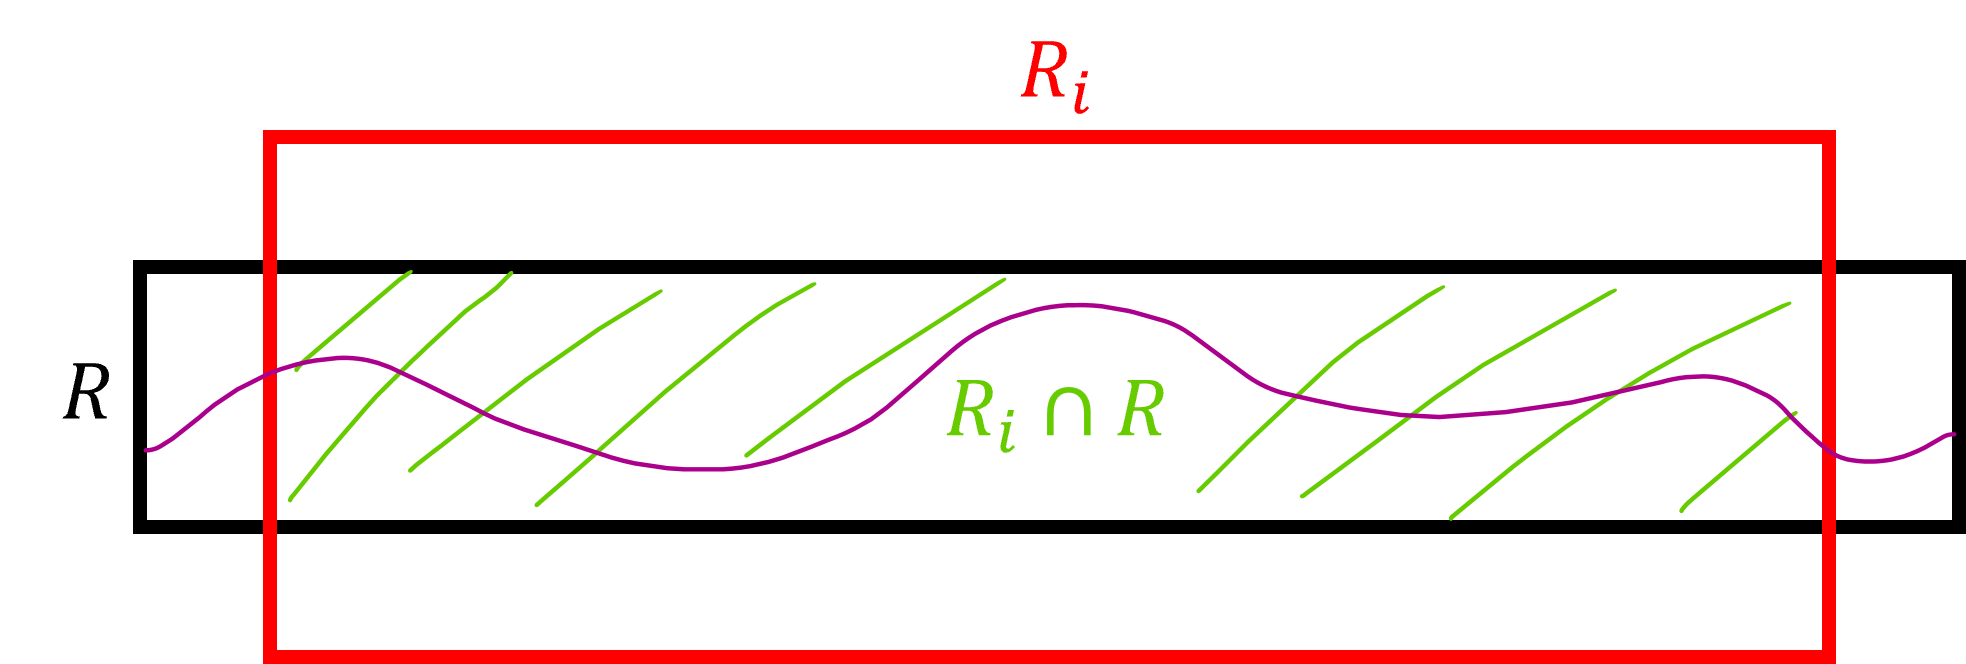
\includegraphics[scale=0.8]{drawings/rectangleOverlap.png}
		\caption{An example $14n$ by $2n$ rectangle in black, with overlapping $12n$ by $4n$ rectangle $R_i$ in red. The $12n$ by $2n$ rectangle induced by their intersection is shaded in green. The purple open horizontal crossing in $R$ clearly implies an open horizontal crossing in $R_i$.}
		\label{fig:rectangleOverlap}
	\end{figure}

	Then for each $i$ we can take complements of Harris' Lemma (Lemma~\ref*{harrisLemma}) to see that the decreasing events $E^c_{n,i}$ and $\cap_{j<i}E^c_{n,j}$ are positively correlated. Thus we see,
	$$\probtorus(E^c_n) \geq \probtorus\left(\bigcap^{128}_{i=1}E^c_{n,i}\right) \geq \prod_{i=1}^{128}\probtorus(E^c_{n,i}) = \probtorus(E^c_{n,1})^{128}$$
	Where we have repeatedly applied Harris' Lemma to get the second inequality.
	Now combining this with our earlier result that $\probtorus(E_n) \geq 1-n^{-128 \delta}$, we find that for $n> n_0$:
	$$\probtorus(E_{n,1}^c) \leq \probtorus(E_n^c)^{1/128} \leq n^{- \delta}$$
	Hence,
	$$\probtorus(E_{n,1}) \geq 1- n^{- \delta}$$
	Since $E_{n,1}$ is the event there is an open horizontal crossing of a $12n$ by $4n$ rectangle, say $R$, in $\mathbb{T}_{16n}$. Then by our previous reasoning $R$ has a corresponding $12n$ by $4n$ rectangle $R'$ in $\ints^2$. 
	Hence, we get our final result for $n>n_0$ that:
	$$\prob(H(R')) = \probtorus(H(R)) \geq 1-n^{-\delta}$$
\end{proof}

Using this lemma we are in a position to prove Kesten's Theorem, for the proof we follow the method outlined in \cite{bollo2006}.

\begin{theorem}[Kesten's Theorem]
	For Bernoulli bond percolation on $\ints^2$, if $p>1/2$ then $\theta(p) > 0$
\end{theorem}

\begin{proof}
	Let $p >1/2$, and define $\delta = \delta(p)$ and $n_0 = n_0(p,2)$ as in Lemma~\ref*{kesternLemma}. Initially suppose some integer $n$ such that $n > n_0$, we will put further constraints on $n$ later. Then for $k = 0,1,2,3,...$ define $R_k$ to be the rectangle with side lengths $2^{k}n$ and $2^{k+1}n$, with the longer side vertical if $k$ is even and horizontal otherwise. We position the bottom left corner of all $R_k$ rectangles at the origin so that $R_i$ encloses $R_{i-1}$, see Figure~\ref*{fig:KesternRectangle}.

	\begin{figure}
		\centering
		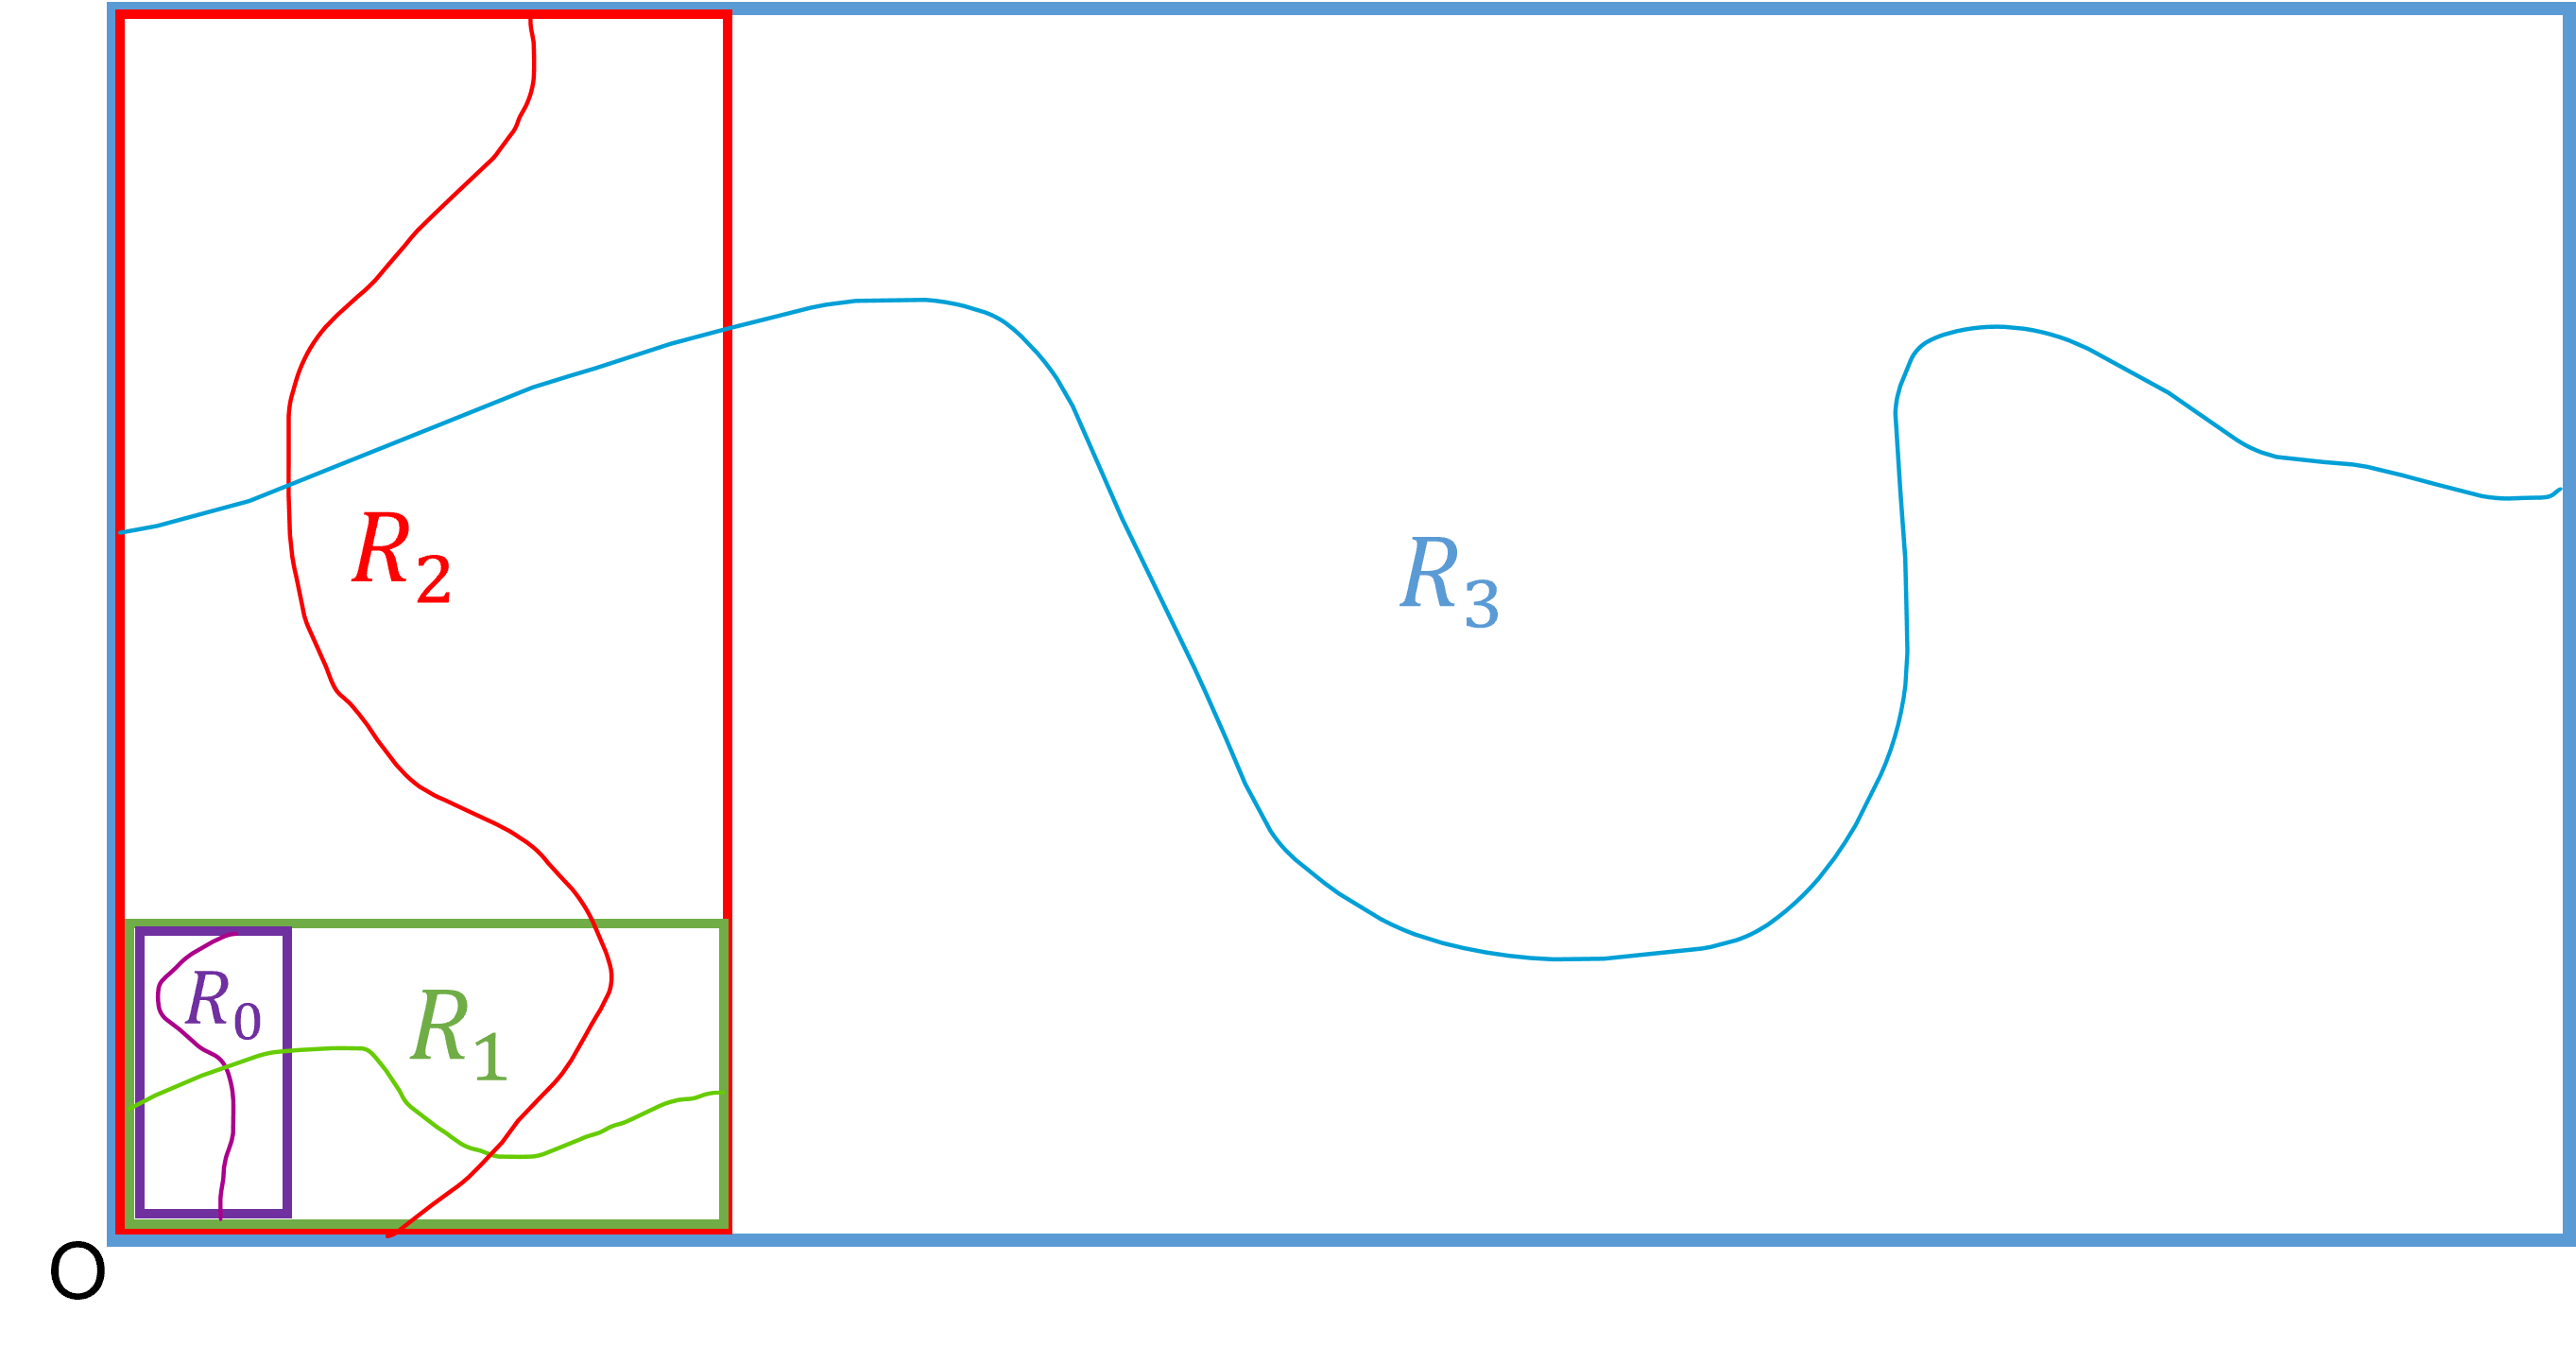
\includegraphics[scale=0.58]{drawings/kestenRectangles.png}
		\caption{Rectangles $R_k$ for $k=0,1,2,3$ with their open crossings corresponding to all $E_k$ holding. $R_0$ in purple, $R_1$ in green, $R_2$ in red and $R_3$ in blue.}
		\label{fig:KesternRectangle}
	\end{figure}

	Let $E_k$ be the event that $R_k$ admits an open crossing of edges the long way. Clearly if $E_k$ and $E_{k+1}$ hold then the open crossings of $R_k$ and $R_{k+1}$ must meet, as depicted in Figure~\ref*{fig:KesternRectangle}. Then using Lemma~\ref*{kesternLemma} and the formula for infinite geometric series we see that,
	$$\sum_{k=0}^{\infty}\prob(E^c_k) \leq \sum_{k=0}^{\infty}(2^kn)^{-\delta} = \frac{n^{-\delta}}{1-2^{-\delta}}$$
	Clearly we can require $n$ to be large enough such that,
	$$\sum_{k=0}^{\infty}\prob(E^c_k) \leq  \frac{n^{-\delta}}{1-2^{-\delta}} < 1$$
	Which implies that $$\prob\left(\bigcap_{k=0}^{\infty}E_k\right)>0$$
	Now if $E_k$ holds for all $k$ then the event,$E_{\infty}$, that there is an infinite open cluster must also hold. Thus,
	$$\prob(E_{\infty}) \geq \prob\left(\bigcap_{k=0}^{\infty}E_k\right)>0$$
	Attentive readers may note that while $E_{\infty}$ implies there is an infinite open path, this path may not necessarily start at the origin. However clearly the probability of an open path from the origin along the bottom edge of $R_0$ is positive, thus when $p>1/2$ we have $\theta(p) >0$. 

\end{proof}
It may interest the reader to know that the final step in the proof is not strictly necessary, the event that there is an infinite open cluster containing the origin is translation invariant. This means that probability of an infinite cluster is not affected by a shift in edge configurations. We not do prove this property here, but the reader may wish to see \cite{duminil2018introduction} for details. 

Furthermore, the event that there is an infinite open cluster in the lattice is an example of a tail event, since clearly it is independent of the configuration of any finite number of edges. Thus, Kolmogorov's 0-1 law can be applied to this event. We take the definition from \cite{bollo2006}.
\begin{theorem}[Kolmogorov's 0-1 law]\label{01Law}
	Let $X = (X_1,X_2,...)$ be a sequence of independent random variables, and let $A$ be an event generated by the \sigalg generated by $X$. Suppose that for all $n$, the event $A$ is independent of $X_1,...,X_n$. Then, $$\mathbb{P}(A) \in \{0,1\}.$$
\end{theorem}
This theorem immediately tells us when the square lattice admits an infinite open cluster. 

\begin{corollary}
	By Theorem~\ref*{01Law}, we have 
	$$\prob(E_{\infty}) = \begin{cases}
		0 & \text{if }p \leq 1/2\\
		1 & \text{if }p > 1/2\\
	\end{cases} $$
\end{corollary}

% \section{Conformal Invariance}
% Discuss what conformal invariance is and perhaps talk about the result on the triangular lattice due to Smirnov

\section{Simulation}
In this section we discuss techniques and algorithms which can be used to explore percolation via simulations. We aim to outline a general method to investigate the critical crossing probability of finite boxes in such a way that it can be applied to any graph with minimal modification. We use the analytical proof for the critical value on the square lattice presented in Section~\ref*{HarrisKesten} to verify correctness of our method.
\subsection{The ``water level'' of open crossings in finite boxes}
% {\color{red}{Discuss how uniform R.V.s can be assigned to edges to simulate percolation. 
% Then plot the threshold for open crossings across some size box. 
% Then see the sharpening of said plot when the box size increases.}}

As we have seen previously the task of determining the percolation threshold for a given lattice structure is highly non-trivial and so for many lattices the task of finding exact values is still an open problem \cite{StoverThreshold}. Subsequently, a great deal of work has been carried out to determine approximate values for a variety of lattices and distributions of open sites or bonds by way of computer simulations. In this section we explore a method I used to estimate the bond percolation threshold for the square lattice, since we can compare this to the exact value of $1/2$ we proved earlier. 

While we know that the fact that a configuration having an open crossing from one side to another of a single finite box in $\ints^2$ does not affect the probability of there being an infinite connected cluster. It is clear that we would expect the probability of such a crossing in a very large box to tend towards the percolation threshold for the infinite cluster. Hence, we can exploit this behaviour to find an estimate for the percolation threshold, create some large square grid, assign some configuration of open and closed edges with probability $p$, then check for a left-right crossing. We alter the value of $p$ repeatedly until we find the lowest value at which a crossing occurs.

There are a number of factors to consider when setting up this simulation such that it can run sufficiently fast, firstly how do we assign each edge to be open or closed so that we can traverse the graph with different values of $p$.

The simplest approach would be to assign a Bernoulli random variable with probability $p$ to each edge, however this has the drawback of requiring us to revaluate the random variable on each edge when we change the value of $p$, and to mirror the non-decreasing nature of the percolation function $\theta(p)$, we would have to only do this for previously closed edges. To avoid these issues I chose to implement a method similar to one we used to prove Lemma~\ref{incEventlemma}, where we coupled configurations using uniform random variables. To recap this, by assigning an edge with a value from independent uniform random on $[0,1]$ we can then set an edge to be open if this value is less than or equal to $p$ and closed otherwise. In this way every edge is open with probability $p$, and increasing p has the desired property that edges which were previously open remain so. Additionally, after the values between 0 and 1 have been assigned to each edge, we gain the benefit of only needing to query the state of edges as we come to them by comparing the assigned value to $p$, rather than needing to assign the open or closed states to every edge each time we alter $p$.

We could remove the initial pass of assigning the uniform random variable values to each edge initially. Instead, we could define some hash function mapping the existing attributes of each edge to the range $[0,1]$, allowing us to compute the states of edges on the fly. However, I did not find this speed up necessary.

Secondly how do we check quickly for a given box if there is a left-right crossing. The first step in simplifying this problem to add two auxiliary vertices to the graph, one connected to every vertex on the left-hand side of the box, the other to the right-hand side vertices. Then our problem reduces to whether there is a path between these two auxiliary vertices via open edges.
The fastest way to go about this, since we have an unweighted graph, is to use a version of breadth first search. Taking the subgraph induced by the open edges, note we always set edges incident to the auxiliary edges to be open, we follow a simple algorithm.
\begin{algorithm}
	\caption{Breadth first search from vertex u to v}\label{bfs}
	\begin{algorithmic}[1]
	\Procedure{bfsPath}{$G,u,v$}
	\State{\textbf{Let} $Q$ be a queue}
	\State{\textbf{Let} $explored$ be a list of booleans}
	\State{\textbf{Let} $parent$ be a list of nodes}
	\State{$explored[u] \gets$ True}
	\State{$parent[u] \gets$ None}
	\State $Q$.enqueue($u$)
	\While{$Q$ is not empty}
		\State $x \gets Q\text{.dequeue()}$
		\If {$x$ is $v$} \Comment{Retrace parents to find path}
			\State $path \gets [x]$
			\While{$parent[x]$ is not None}
				\State $path$.prepend(parent[$x$])
				\State $x \gets parent[x]$
			\EndWhile
			\State
			\Return $path$
		\EndIf
		\For{every edge $w$ in $G$.adjacent($x$)}
			\If{$explored[w]$ is False}
				\State $explored[w] \gets$ True
				\State $parent[w] \gets$ $x$
				\State $Q$.enqueue($w$)
			\EndIf
		\EndFor
	\EndWhile
	\If{$explored[v]$ is False}
	 \Return None
	\EndIf
	\EndProcedure
	\end{algorithmic}
	\end{algorithm}

We note a queue is a simple data structure which works in the same way as a queue at a shop. The first item added to the queue is the first to then be removed.
The above algorithm runs in $O(|V|+|E|)$ worst-case time, where $V$ and $E$ are the vertex and edge sets of the graph $G$ respectively. With a little thought it is clear no algorithm can do better for this problem. 

We also note that Algorithm~\ref*{bfs} returns the list of nodes on the path between the two vertices. Depending on the use case this can be easily modified to just return true if a path exists. 

Now we can determine if there is a path from one side of a box to another for a given percolation parameter $p$, we want to determine the lowest threshold for which a crossing path exists for a given configuration of uniform random variables. For the case of the planar square lattice we could use some heuristic based on our prior knowledge that the threshold should lie around 1/2. However, to enable the general applicability of the algorithm described to any graph, we do not make any specific assumptions about the threshold distribution.

While a variety of possible approaches exist, a rather efficient one is an adapted form of binary search on the parameter. While usually a binary search can be used to identity sorted items in a list, in some sense our parameter values are also sorted. All the values with a left right crossing appear before those which do have a crossing, this is only true due to our implementation via uniform random variables on each edge.
In order to check if a given value of $p$ is the crossing threshold, we must check a value very close to $p$ to see if it is different. Say we have some precision constant $\epsilon$ then we define:
\begin{itemize}
	\item If $p$ admits a box crossing, then $p$ is the crossing threshold if and only if $p-\epsilon$ does not.
	\item If $p$ does not admit a box crossing, then $p+\epsilon$ is the crossing threshold if and only if $p+\epsilon$ does admit a crossing.
\end{itemize}

Now we can follow an adapted binary search to centre in on the threshold, where we let isPath(G, u, v) be the aforementioned change to Algorithm~\ref*{bfs} so that it returns a boolean value.

\begin{algorithm}
	\caption{Find the crossing threshold for a given graph}\label{findthreshold}
	\begin{algorithmic}[1]
	\Procedure{findThreshold}{$G,u,v,\epsilon$} \Comment{u \& v are the auxiliary nodes}
	\State lo $\gets 0$
	\State hi $\gets 1$
	\While{lo $\leq$ hi}
		\State $p \gets (\text{lo}+\text{hi})/2$
		\State openEdges $\gets$ $\{e \in E(G)\text{: e has uniform r.v. value}\leq p\}$
		\State \textbf{let} OpenG be the subgraph of G induced by openEdges
		\If{isPath(openG, u, v)}
			\State altOpenEdges $\gets$ $\{e \in E(G)\text{: unifRV}(e)\leq p-\epsilon\}$
			\State \textbf{let} AltG be the subgraph of G induced by altOpenEdges
			\If{isPath(AltG, u, v)}
				\State hi $\gets p - \epsilon$
			\Else
				\State \Return $p$
			\EndIf
		\Else
			\State altOpenEdges $\gets$ $\{e \in E(G)\text{: unifRV}(e)\leq p+\epsilon\}$
			\State \textbf{let} AltG be the subgraph of G induced by altOpenEdges
			\If{isPath(AltG, u, v)}
				\State \Return $p +\epsilon$
			\Else
			\State lo $\gets p+\epsilon$
			\EndIf
		\EndIf
	\EndWhile
	\EndProcedure
	\end{algorithmic}
\end{algorithm}

You can inspect the above algorithm to see how whenever the current value of $p$ is not the threshold we can safely throw out one half of the current search range. This technique, commonly referred to as divide and conquer, gives good asymptotic search performance. We would say in general a binary search finds the target in $O(nlog(n))$ worst-case time where n is the number of elements to be searched. In our case the effective number of ``items'' depends on the precision parameter $\epsilon$, where the number of potential threshold values to check is $\frac{1}{\epsilon}$. Thus Algorithm~\ref*{findthreshold} runs in $O(\frac{1}{\epsilon}log(\frac{1}{\epsilon}))$ worst-case time.

You may notice a possible optimization when both the algorithms are used together. Instead of first constructing the induced subgraph by the open edges then seeing if there is a crossing, we can directly only consider the open edges during our breadth first search by requiring in line 18 of Algorithm~\ref*{bfs} that the edges $w$ must have associated uniform random variable value of less than or equal to p. In essence, we can construct the subgraph induced by the open edges on the fly, saving us one pass over the edge set. 

My initial plan to investigate the percolation threshold for the planar square lattice was to simulate many boxes each of increasing width to see how the variation in the crossing threshold decreases with box width. Using the previously described algorithms to find the threshold for each box.

I implemented the simulation using Python due to its extensive set of community libraries and ease of prototyping. Since Python is an interpreted language it can be less performant than other complied languages which can be an important consideration for very large simulations. However, alternative interpreters  of Python such as PyPy can mitigate this issue \cite{PyPy}. PyPy uses just-in-time compilation and other optimization techniques to speed up native python code.
I decided to simulate one box of each width from width 2 (3x3 vertices) to width 1950, with a precision of $0.0001$. I then used the matplotlib library to draw a scatter plot of the box width against the computed crossing threshold, which can be seen in Figure~\ref*{fig:thresholdplot2}. The red dashed line lies at the threshold value 0.5 which we know is the true value for an infinite lattice.

\begin{landscape}
	\begin{figure}
		\centering
		\makebox[3\textwidth][l]{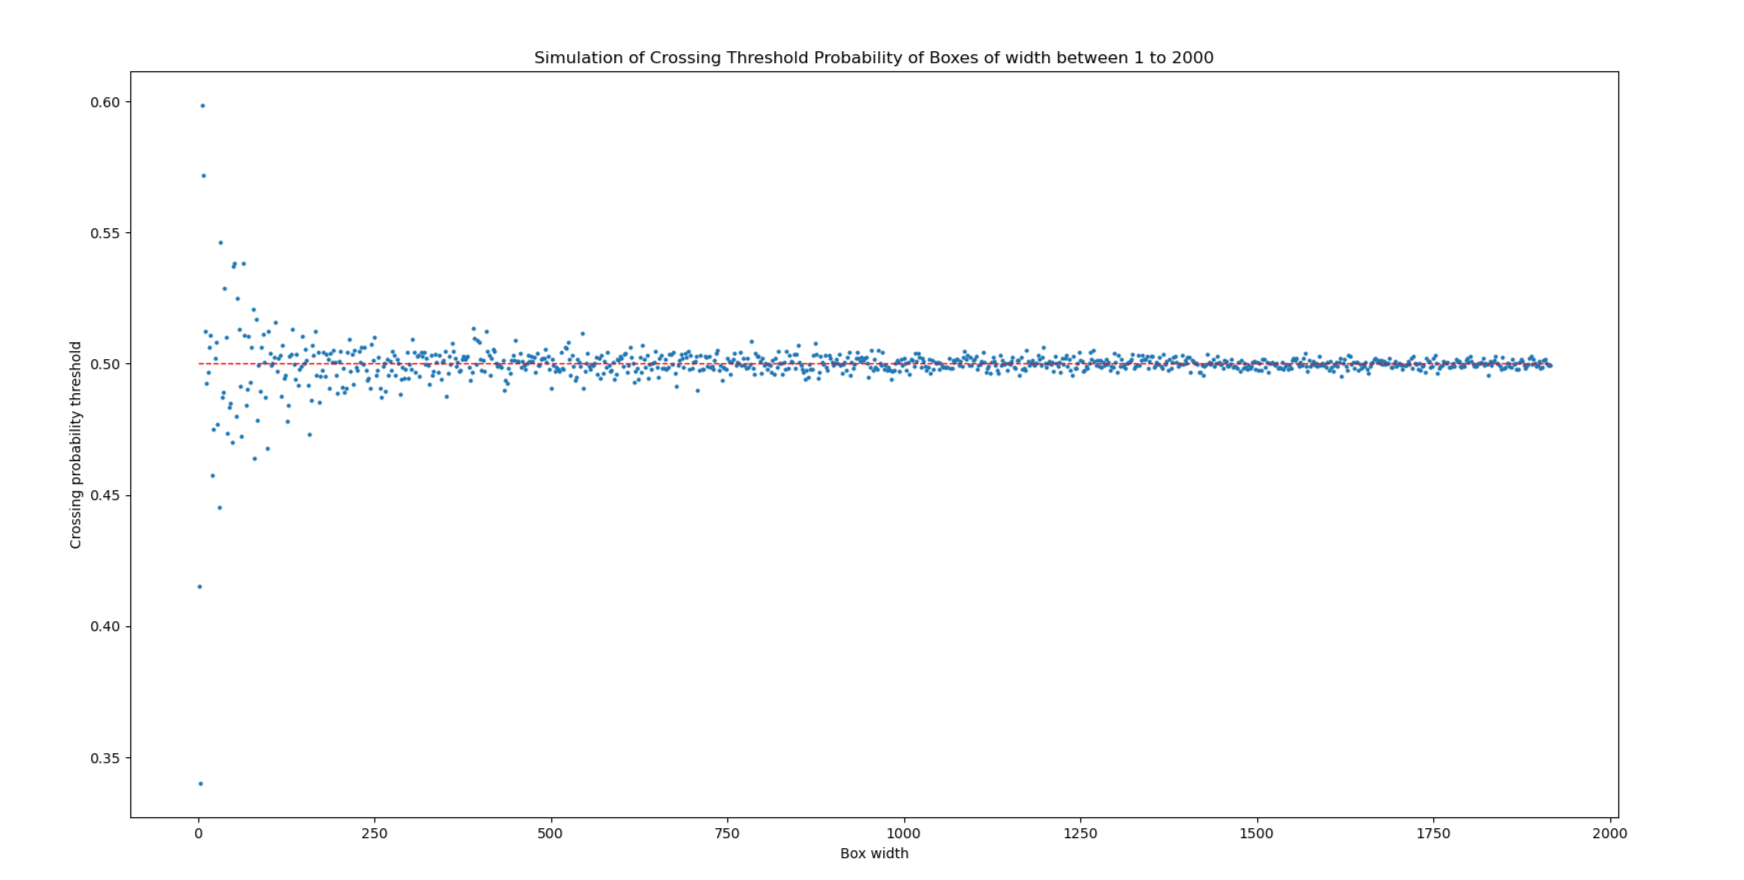
\includegraphics[scale=0.58]{CrossingSimulationPlot3.png}}
		\caption{Crossing thresholds for simulated lattices}
		\label{fig:thresholdplot2}
	\end{figure}
	\end{landscape}

You can clearly see how the variability of crossing threshold decreases as the box width increases, becoming more concentrated around 0.5. Supposing we did not already know the true value of the infinite lattice, this would provide us with a strong insight that the percolation threshold lies around 0.5. In fact if we calculate the mean of the crossing thresholds for each box, disregarding the first 50 due to their small size, we would get a value of 0.499979 which when rounded to our precision of 0.0001 is 0.5000.

This verifies the method we have used as giving a good approximation for the percolation threshold. Since no part of our simulation or algorithm depended on specific structure of the square planar lattice, it would be very easy to use this approach to investigate other planar graph structures. In fact, with some adaptations the Algorithm~\ref*{bfs} could be extended to consider an $n$-dimension hypercube to allow the investigation of Bernoulli percolation on arbitrary dimension lattices. Further to this we can easily assign values from different random distributions to each edge, and explore how this affects the crossing threshold.

% \begin{figure}
% 	    \centering
% 	    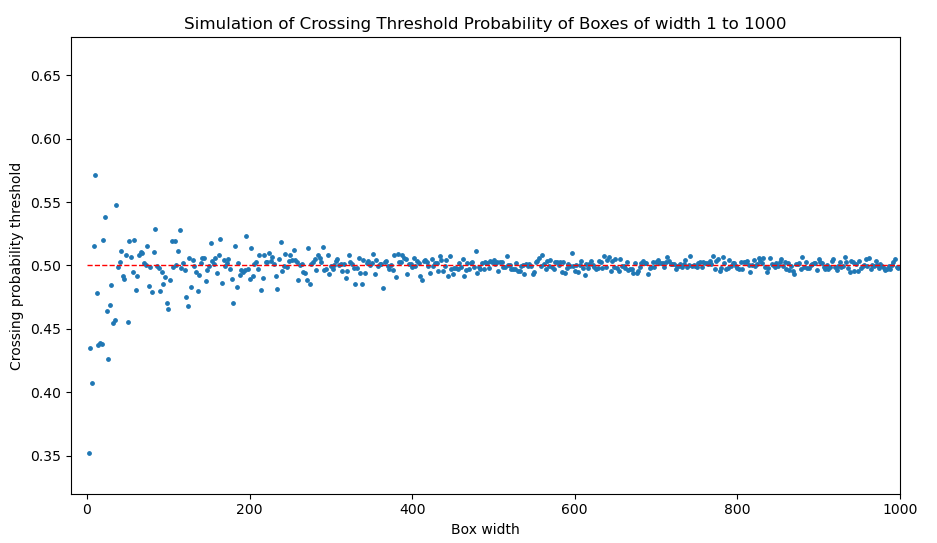
\includegraphics[scale=0.52]{CrossingSimulationPlot2.png}
% 	    \caption{Crossing thresholds for simulated lattices}
% 	    \label{fig:thresholdplot}
% \end{figure}



% \subsection{Finding the pivotal edges in a finite box}
% Discuss an algorithm to find the pivotal edges in the percolation box, perhaps relate to Russo's formula for pivotal edges.
% \subsection{Fast Monte Carlo algorithm for percolation}
% Discuss the Newman and Ziff paper "A fast Monte Carlo algorithm for site or bond percolation". Explaining the data structures etc, and perhaps implement it.

% \section{Conclusion}
% Is a conclusion necessary for this project?


\printbibliography

\section{Appendix}
Below is the Python code I used to carry out my simulations:

\begin{minted}[tabsize=3,xleftmargin=-80pt]{python}
	import networkx as nx
	import random
	import time
	
	def gen2dLattice(n):
		'''Create a 2n by 2n square graph'''
		return nx.grid_2d_graph(range(-n,n+1),range(-n,n+1))
	
	def percGraph(n):
		G = gen2dLattice(n)
		num_edges = nx.number_of_edges(G)
		unifRvs = [random.random() for _ in range(num_edges)]
		# Create Dictionary from edges to their unif rv
		dictUnifRvs = {coord:rv for coord,rv in zip(G.edges,iter(unifRvs))} 
		# bind the unif rvs to the edges in the graph 
		nx.set_edge_attributes(G,dictUnifRvs,name="unifRv") 
		#create aug graph with s and f nodes which connect to the left an right sides resp
		GAug = G.copy()
		GAug.add_node('s') 
		GAug.add_node('f')
		for i in range(-n,n+1): # Add the edges to s and f
			GAug.add_edge('s',(-n,i))
			GAug.add_edge((n,i),'f')
		return G , GAug
	
	def find_crossing_path(openEdges,GAug) -> list:
		'''finds left/right crossing by open edges if one exists
		Returns: List of edges on the path'''
		 # find the subgraph of open edges plus the aux left right edges
		GOpen = nx.edge_subgraph(GAug,list(GAug.edges('f')) 
			+ list(GAug.edges('s')) 
			+ [(e[0],e[1]) for e in openEdges])
		edgepath = []
		try:
			openPaths = nx.algorithms.shortest_paths.bidirectional_shortest_path(GOpen,'s','f')
		except:
			#If no path is found
			openPaths = []
		for i in range(len(openPaths)): #Convert from list of nodes to list of edges
			edgepath.append((openPaths[i-1],openPaths[i]))
		openPaths = edgepath
		return openPaths
	
	def find_threshold_binary_search(i,precision):
		'''Finds the threshold for a left right crossing on a 2i x 2i box'''
		G, GAug = percGraph(i)
		lo=0
		hi=1
		p = (lo+hi)/2
		openEdges = [e for e in G.edges(data=True) if e[2]['unifRv']<=p]
		crossing = find_crossing_path(openEdges, GAug)
		while lo <= hi:
			p = (lo+hi)/2
			openEdges = [e for e in G.edges(data=True) if e[2]['unifRv']<=p]
			crossing = len(find_crossing_path(openEdges, GAug))
			if crossing == 0:
				pAlt = p + precision
				openEdgesAlt = [e for e in G.edges(data=True) if e[2]['unifRv']<=pAlt]
				crossingAlt = len(find_crossing_path(openEdgesAlt, GAug))
				if crossingAlt >0:
					return pAlt
				else:
					lo = pAlt    
			else:
				pAlt = p - precision
				openEdgesAlt = [e for e in G.edges(data=True) if e[2]['unifRv']<=pAlt]
				crossingAlt = len(find_crossing_path(openEdgesAlt, GAug))
				if crossingAlt ==0:
					return p
				else:
					
					hi = pAlt
		return 'Error'
	
	start_time = time.time()
	thresholds = [find_threshold_binary_search(i,0.0001) for i in range(1,1000)]
	print(thresholds)
	end_time = time.time()
	print(f"It took {end_time-start_time:.2f} seconds to compute")
	
\end{minted}

\end{document}